\setcounter{chapter}{4}

\chapter{定积分}

定积分和不定积分在概念上是截然不同的,二者通过微积分基本定理建立起
联系,这种联系体现了积分和微分的相对关系。

在现实问题中,定积分有着非常广泛的应用,很多求面积、体积的几何问题
以及众多的物理问题都可以化为定积分来计算。

\section{定积分的概念与性质}

\subsection{定积分的概念}

和导数一样,定积分是用极限来定义的。

为了解释其概念,我们从一个典型的问题出发,即所谓的曲边梯形的面积问题。

{\bf 曲边梯形:}由$x$轴,$x=a,x=b$以及曲线$y=f(x)$所围的平面区域。

\begin{center}
	\resizebox{!}{5.2cm}{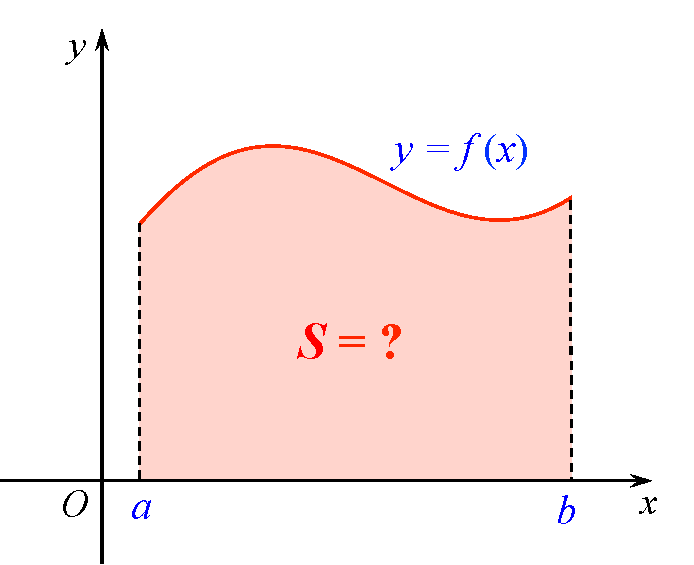
\includegraphics{./images/ch6/integral.pdf}}
	
	$$S=\dint_a^bf(x)\d x$$
\end{center}

求解这个问题的基本思想可以概括为一句话:{\kaishu 分割取近似,做和求极限},也即:

\begin{enumerate}
  \setlength{\itemindent}{1cm}
  \item {\kaishu 分割}:将积分区间$[a,b]$分割成一些列相邻的小区间$[x_{k-1},x_k],
  (k=1,2,\ldots,n)$,其中
  $$a=x_0<x_1<x_2<\ldots<x_{n-1}<x_n=b,$$
  相应地,曲边梯形可以被垂直分割为一系列小的曲边梯形$S_k(k=1,2,\ldots,n)$;不难看出,曲边梯形的
  面积等于所有小的曲边梯形的面积之和$S=\sum\limits_{k=1}^nS_k$;
  \item {\kaishu 取近似}:为了近似表示每个小曲边梯形的面积,任取一个$\xi_k\in
  [x_{k-1},x_k]$,记$\Delta_k=x_k-x_{k-1}$, 则:
  $$S_k\approx f(\xi_k)\Delta_k,$$
  \item {\kaishu 做和}:将所有经过近似的小曲边梯形面积加起来,则为曲边梯形面积的一个近似
  $$S=\sum\limits_{k=1}^nS_k\approx\sum\limits_{k=1}^nf(\xi_k)\Delta_k.$$
  \item {\kaishu 取极限}:为了使对$S$的近似尽可能精确,应考虑将区间$[a,b]$尽可能地
  细分,为此记$\lambda=\max\limits_{1\leq k\leq n}\Delta_k$,然后考虑$\lambda\to0$
  时的极限
  $$I=\lim\limits_{\lambda\to0}\sum\limits_{k=1}^nf(\xi_k)\Delta_k.$$
\end{enumerate}

\begin{thx}
	若对于{\kaishu 任意}的区间分法和近似点取法,以上极限都存在且相同,则称{\bf 函数$f(x)$
	在$[a,b]$上Riemann可积},该极限的值称为{\bf $f(x)$在$[a,b]$上的定积分},
	记为
	$$I=\dint_a^bf(x)\d x.$$
\end{thx}

在以上的定义中,因为包含两个“任意”,因此要以其来判定某个函数的可积性,往往是
非常困难的。幸运的是,在实际应用中,我们可以利用如下的结论来判定一些常用的函数
的可积性:

\begin{thx}
	\begin{enumerate}
	  \item 初等函数在其定义的闭区间上总是可积的;
	  \item 分段连续(只有有限多个第一类间断点)的函数是可积的。
	\end{enumerate}
\end{thx}

% {\bf 例:}求由曲线$y=x^2$以及直线$x=0,x=1$和$y=0$所围成的曲边梯形的面积。

{\bf 例:}证明:Dirichlet函数在任意的区间$[a,b]$上不可积。

{\bf 例:}证明:只改变函数在有限个点处的函数值,其定积分不变,或:
若函数$f(x)$和$g(x)$在$[a,b]$上仅有有限多个点处的函数值相同,
且$f(x)$在$[a,b]$上可积,则$g(x)$也在$[a,b]$上可积,且
$$\dint_a^bf(x)\d x=\dint_a^bg(x)\d x.$$

这个例子的一个直接推论是:若函数$f(x)$在$[a,b]$上仅有有限多个
点处的函数值不为零,则$\dint_a^bf(x)\d x=0$。

\subsubsection{可以化成定积分的极限问题}

当函数$f(x)$在$[a,b]$上可积时,其定积分的值不因区间分法和近似点的取法
而不同,特别地,可以考虑其中对区间进行平均分割和取区间端点为近似点的情形
来构造一些特殊的极限问题:

\begin{thx}
	若$f(x)$在$[a,b]$上可积,则
	$$\dint_a^bf(x)\d x
	=\limn\sum\limits_{k=1}^nf\left[a+\df kn(b-a)\right]\df{b-a}n.$$
\end{thx}

这相当于对区间$[a,b]$做了$n$等分,然后取分割后的区间端点$a+\df kn(b-a)$
作为近似点。特别地,当积分区间为$[0,1]$时,有
$$\dint_0^1f(x)\d x=\limn\sum\limits_{k=1}^nf\left(\df kn\right)\df1n.$$

{\bf 例:}将下列极限表示成定积分:
\begin{enumerate}[(1)]
  \setlength{\itemindent}{1cm}
  \item $\limn\df 1n\left[\sin\df{\pi}{n}+\sin\df{2\pi}{n}+\ldots
  +\sin\df{(n-1)\pi}{n}\right]=\df1{\pi}\dint_0^{\pi}\sin x\d x=\df2{\pi}$ 
  \item $\limn\left(\df{1}{n^2}+\df{2}{n^2}+\ldots+\df{n-1}{n^2}\right)
  =\dint_0^1x\d x=\df12$
  \item $\limn\sum\limits_{k=1}^n\df{k}{n^3}\sqrt{n^2-k^2}
  =\dint_0^1x\sqrt{1-x^2}\d x=\df13$
\end{enumerate}

{\bf 例:}$G_n=\sqrt[n]{(n+1)(n+2)\cdots(n+n)},(n=1,2,\ldots)$,求
$\limn\df{G_n}n$.

[提示]:
$$\ln\df{G_n}n=\limn\df1n\sum\limits_{k=1}^n\ln\left(1+\df kn\right)
=\dint_0^1\ln(1+x)\d x=2\ln2-1$$

\begin{shaded}
{\bf 例:}利用定积分定义证明以下极限:
$$\limn\cos\df x2\cos\df x4\cos\df x8\cdot\cdots\cdot\cos\df x{2^n}
=\df{\sin x}x,$$
并证明Vieta's Formula(韦达公式)
$$\df2\pi=\df{\sqrt2}2\cdot\df{2+\sqrt2}2\cdot\df{\sqrt{2+\sqrt{2+\sqrt2}}}2
\cdot\cdots$$

[提示]:
\begin{align}
	&\cos\df x2\cos\df x4\cos\df x8\cdots\cos\df x{2^n}\notag\\
	&=\df12\left(\cos\df34x+\cos\df14x\right)\cos\df x8\cdots\cos\df
	x{2^n}\notag\\
	&=\df1{2^2}\left(\cos\df78x+\cos\df58x+\cos\df38x+\cos\df18x\right)
	\cos\df x{16}\cdots\cos\df x{2^n}\notag\\
	&=\ldots\notag\\
	&=\df1{2^{n-1}}\left(\cos\df{2^n-1}{2^n}x+\cos\df{2^n-3}{2^n}x+
	\ldots+\cos\df3{2^n}x+\cos\df1{2^n}x\right)\notag\\
	&=\dint_0^1\cos(xt)\d t=\df{\sin x}x\notag
\end{align}
\end{shaded}

\subsection{定积分的几何意义}

\begin{center}
	\resizebox{!}{3.12cm}{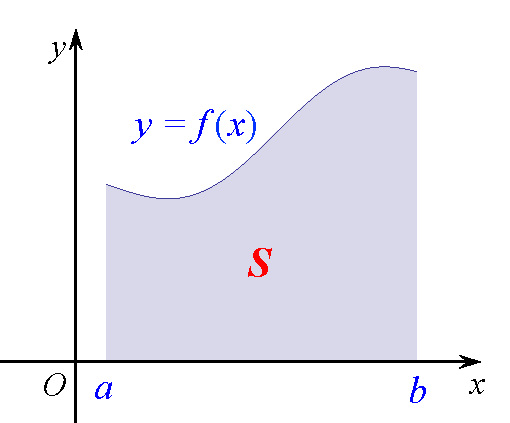
\includegraphics{./images/ch6/IS1.pdf}} 
	\resizebox{!}{3.12cm}{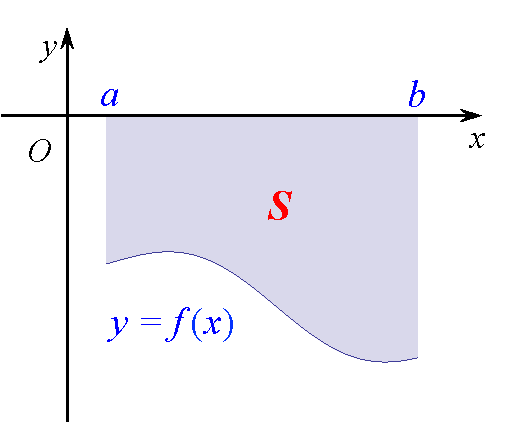
\includegraphics{./images/ch6/IS2.pdf}} 
	\resizebox{!}{3.12cm}{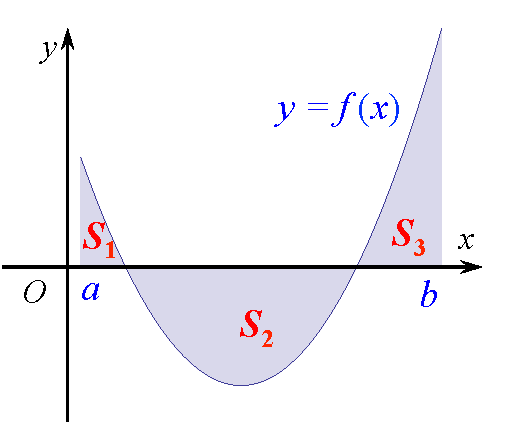
\includegraphics{./images/ch6/IS3.pdf}}
	
	{\b\it “定积分表示的是带符号的面积” }
\end{center}

为了定积分计算的方便,我们作出如下的约定:
\begin{thx}
	\begin{enumerate}
% 	  \setlength{\itemindent}{1cm}
	  \item $\dint_a^af(x)\d x=0$
	  \item $\dint_b^af(x)\d x=-\dint_a^bf(x)\d x$ 
	\end{enumerate}
\end{thx}

\subsection{定积分的基本性质}

\begin{thx}
	\begin{enumerate}[(1)]
% 	  \setlength{\itemindent}{1cm}
	  \item {\kaishu 线性性:}
	  $$\dint_a^b[\alpha
	  f(x)+\beta g(x)]\d x=\alpha\dint_a^bf(x)\d x+\beta\dint_a^bg(x)\d x$$
	  \item {\kaishu 区间可加性:}
	  $$\dint_a^bf(x)\d x=\dint_a^cf(x)\d x+\dint_c^bf(x)\d x$$
	  \item {\kaishu 保号性:}%\ps{不定积分不具有保号性!}
	  \begin{itemize}
	    \item $f(x)$在$[a,b]$上可积,且$f(x)\geq 0$,则$\dint_a^bf(x)\d x\geq 0$ 
	    \item $f(x)$在$[a,b]$上连续,非负且不恒为零,则$$\dint_a^bf(x)\d x> 0$$ 
	    \item {\kaishu 保序性:}设$f(x),g(x)$在$[a,b]$上可积,且$f(x)\leq g(x)$,则
	    $$\dint_a^bf(x)\d x\leq \dint_a^bg(x)\d x$$
	    \item {\kaishu 绝对值不等式:}$f(x)$在$[a,b]$上可积,则
	    $${\b \dint_a^bf(x)\d x\leq\dint_a^b|f(x)|\d x}$$ 
	    \item {\kaishu 积分估值:}$f(x)$在$[a,b]$上可积,且$m\leq f(x)\leq M$,则
	    $$m(b-a)\leq\dint_a^bf(x)\d x\leq M(b-a)$$
	  \end{itemize}
	\end{enumerate}
\end{thx}

{\bf 例:}设$I_k=\dint_0^{k\pi}e^{x^2}\sin x\d x$,试比较$I_1,I_2,I_3$
的大小。

\begin{center}
	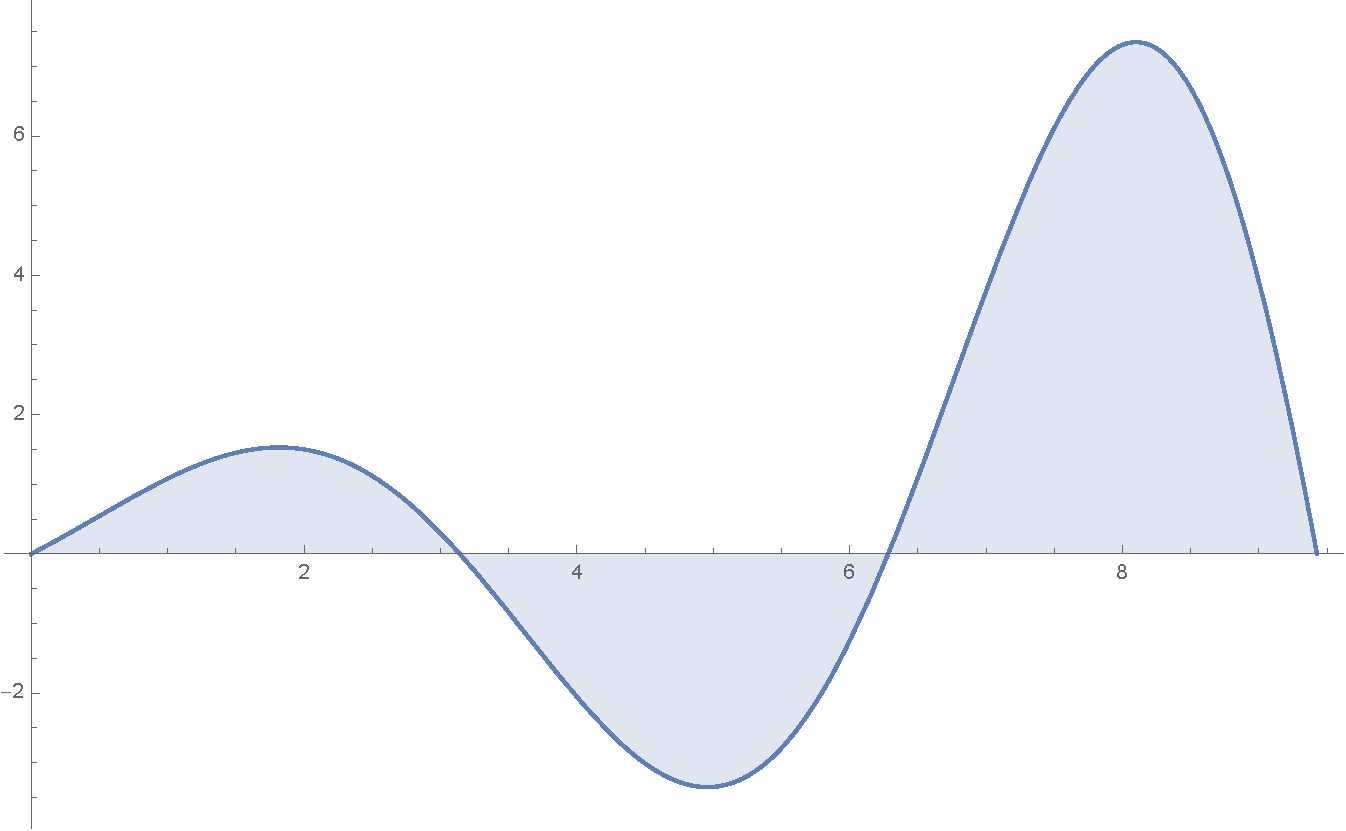
\includegraphics[width=8cm]{./images/ch5/ex2sinx.pdf}
\end{center}

[解]:注意到$e^{x^2}$当$x>0$时严格单调递增,故
$$\dint_0^{\pi}e^{x^2}\sin x\d x
<\dint_{\pi}^{2\pi}e^{x^2}|\sin x|\d x
<\dint_{2\pi}^{3\pi}e^{x^2}\sin x\d x,$$
于是由定积分的区间可加性,可得$I_2<I_1<I_3$。\fin

\subsubsection{用定积分的性质证明不等式}

\begin{thx}
	{\bf Schwarz积分不等式:}设$f(x),g(x)$均在$[a,b]$上连续,证明:
	$$\left[\dint_a^bf(x)g(x)\d x\right]^2
	\leq\dint_a^bf^2(x)\d x\dint_a^bg^2(x)\d x$$
\end{thx}

[证一]:
\begin{align*}
	&\dint_a^bf^2(x)\d x\dint_a^bg^2(x)\d x
	=\dint_a^bf^2(x)\d x\dint_a^bg^2(y)\d y\\
	&=\dint_a^b\dint_a^bf^2(x)g^2(y)\d x\d y
	=\dint_a^b\dint_a^bf^2(y)g^2(x)\d x\d y\\
	&=\dint_a^b\dint_a^b\df12\left[f^2(x)g^2(y)
	+f^2(y)g^2(x)\right]\d x\d y\\
	&\geq \dint_a^b\dint_a^bf(x)g(y)
	f(y)g(x)\d x\d y\\
	&=\dint_a^bf(x)g(x)\d x\dint_a^bf(y)g(y)\d y
	=\dint_a^bf(x)g(x)\d x\dint_a^bf(x)g(x)\d x\\
	&=\left[\dint_a^bf(x)g(x)\d x\right]^2.
\end{align*}
\fin

[证二]:不妨设$\dint_a^bf^2(x)\d x>0$,对任意$t\in\mathbb{R}$
$$\dint_a^b(tf-g)^2\d x=t^2\dint_a^bf^2\d x-2t\dint_a^bfg\d x
+\dint_a^bg^2\d x\geq 0$$
故必有
$$\Delta=\left(\dint_a^bfg\d x\right)^2-\dint_a^bf^2\d x\dint_a^b
g^2\d x<0$$
若$\dint_a^bf^2\d x=\dint_a^b g^2\d x=0$,则
$$\left|\dint_a^bfg\d x\right|\leq\dint_a^b|fg|\d x
\leq\dint_a^b\df12(f^2+g^2)\d x=0.$$
\fin

使用与证法一类似地方法可证明
\begin{thx}
	{\bf Cauchy不等式:}
	$$\left(\sum\limits_{i=1}^na_ib_i\right)^2\leq
	\sum\limits_{i=1}^na_i^2\sum\limits_{i=1}^nb_i^2$$
\end{thx}
积分的实质就是求和,因此Cauchy不等式和Schwarz不等式从本质上是一致的,
因此这两个不等式放在一起,统称{\kaishu Cauchy-Schwarz不等式}。

{\bf 例:}$f(x)\in C[a,b]$,且$f(x)>0$,则
$$\dint_a^bf(x)\d x\dint_a^b\df1{f(x)}\d x\geq(b-a)^2$$

{\bf 例:}设$f(x)$在$[a,b]$上连续可微,$f(a)=0$,证明:
$$\dint_a^b[f(x)]^2\d x\leq\df{(b-a)^2}{2}\dint_a^b[f\,'(x)]^2\d x$$

从Cauchy-Schwarz不等式出发,还可以类似地证明{\kaishu Minkowski不等式}:
$$\left\{\dint_a^b[f(x)+g(x)]^2\d x\right\}^{\frac12}
\leq\left[\dint_a^bf^2(x)\d x\right]^{\frac12}
+\left[\dint_a^bg^2(x)\d x\right]^{\frac12}.$$

\subsection{定积分中值定理}

\begin{thx}
	若函数$f(x)$在区间$[a,b]$上连续,
	则在$[a,b]$上至少存在一点$\xi$,使得
	$$\dint_a^bf(x)\d x=f(\xi)(b-a)$$
\end{thx}

[证]:因为$f(x)$在$[a,b]$上连续,故必存在最大和最小值,分别记为$M$和$m$。
于是,有积分估值定理,可得
$$m\leq\df1{b-a}\dint_a^bf(x)\d x\leq M,$$
进而由连续函数的介值定理,可知必存在某个$\xi\in[a,b]$,使得
$$f(\xi)=\df1{b-a}\dint_a^bf(x)\d x.$$
\fin

{\bf 注:}
\begin{enumerate}[(1)]
  \setlength{\itemindent}{1cm}
  \item 若$f(x)$不是$[a,b]$上的连续函数,定理不成立。请自行构造反例!
  \item  {\it\b $f(\xi)$相当于函数$f(x)$在$[a,b]$上的均值(注意不是中值)},
  这一概念在概率统计中得到了广泛应用!
\end{enumerate}

{\bf 例:}计算如下极限
$$\limx{+\infty}\sqrt[3]x\dint_x^{x+1}\df{\sin t}{t+\cos t}\d t$$

[提示]:不妨设$x>1$,由定积分中值定理,存在$\xi\in(x,x+1)$
$$\left|\sqrt[3]x\dint_x^{x+1}\df{\sin t}{t+\cos t}\d t\right|
=\sqrt[3]x\df{|\sin\xi|}{|\xi+\cos\xi|}\leq\sqrt[3]x\df{1}{x-1}
\to0\;(x\to\infty)$$

\begin{ext}
	{\bf 课后作业}
	
	\begin{enumerate}
	  \item 设$f(x)$在$[a,b]$上非负,当$x\in(a,b)$内$f''(x)>0,f'(x)<0$,
		$I_1=\df{b-a}2[f(b)+f(a)]$,$I_2=\dint_a^bf(x)\d x$,$I_3=(b-a)f(b)$,
		试比较$I_1,I_2,I_3$的大小。
	  \item 设$f(x)\in C[0,1]$,证明:$\dint_0^1f^2(x)\d x\geq
	  \left(\dint_0^1f(x)\d x\right)^2$.
	  \item 设$f(x)\in C[a,b]$,$g(x)>0$,证明:存在$\xi\in[a,b]$,使得
	  $$\dint_a^bf(x)g(x)\d x=f(\xi)\dint_a^bg(x)\d x.$$
	  \item 已知$f(x)$在$[0,\pi]$上连续,$(0,\pi)$内可导,且$f(0)=
	  \dint_0^{\pi}f(x)\sin x\d x=0$,证明:存在$\xi\in(0,\pi)$,
	  使得$f'(\xi)=0$。
	  \item (选作)设$f(x)$在$[0,1]$上连续,在$(0,1)$内可导,且$f(0)\cdot f(1)>0$,
	  $f(1)+\dint_0^1f(x)\d x=0$,证明:存在$\xi\in(0,1)$,使得
	  $f'(\xi)=\xi f(\xi)$。
	\end{enumerate}
\end{ext}

\section{微积分基本公式}

\subsection{微积分基本定理}

在Newton和Leibniz之前,微分和积分的许多个别结果已经得到,但只有当
他们发现了这个公式之后,微积分才统计成了一个整体!

\begin{thx}
	{\bf 微积分基本定理:}设函数$f(x)$在区间$[a,b]$上可积,$F(x)$是
	$f(x)$在$[a,b]$上的一个原函数,则
	$$\dint_a^bf(x)\d x=F(b)-F(a).$$
\end{thx}

[证]:由定积分的定义,对区间$[a,b]$的任意分法和近似点$\xi_k\in[x_{k-1},x_k]$
的任意取法,都有
$$I=\lim\limits_{\lambda\to 0}\sum\limits_{k=1}^nf(\xi_k)\Delta_k.$$
对于分法中的任意区间$[x_{k-1},x_k]\;(k=1,2,\ldots,n)$,由Lagrange中值定理,
都存在$\xi_k\in(x_{k-1},x_k)$,使得
$$F(x_k)-F(x_{k-1})=F'(\xi_k)(x_k-x_{k-1})=f(\xi_k)\Delta_k,$$
从而不妨将以上极限中的近似点都取为满足Lagrange中值定理的$\xi_k$,则
必有
$$I=\lim\limits_{\lambda\to 0}\sum\limits_{k=1}^nf(\xi_k)\Delta_k
=\lim\limits_{\lambda\to 0}\sum\limits_{k=1}^n[F(x_k)-F(x_{k-1})]
=\lim\limits_{\lambda\to 0}[F(x_n)-F(x_0)]=F(b)-F(a).$$
即证。\fin

微积分基本定理(或者叫作Newton—Leibniz公式),使得定积分的计算可以不必
从定义出发(那样无疑是非常繁琐和困难的),而只需利用不定积分先求出被积函数
的原函数,再计算原函数在积分区间端点处函数值的差即可。需要说明的是,由于
有些函数并不存在初等函数形式的原函数(例如:$e^{x^2},\df{\sin x}x$),
因此只能采用数值的方法近似计算其在给定区间上的定积分,这时常常还是要从
定积分的定义出发的(区间分割取得约密则积分结果的精度越高)。

{\bf 例:}计算定积分
\begin{enumerate}[(1)]
  \setlength{\itemindent}{1cm}
  \item $\dint_{0}^{1}x^2 \d x$
  \item $\dint_{-1}^{\sqrt 3}\df 1{1+x^2}\d x$
  \item $\dint_{-1}^{-2}\df 1x\d x$
\end{enumerate}

{\bf 注:}
\begin{itemize}
  \setlength{\itemindent}{1cm}
  \item {\it 可积函数未必有原函数},例如,有第一类间断点的函数都没有统一的原函数,
  但是可以分区间对其进行积分;
  \item {\it 有原函数的函数未必可积},例如:函数
  $$f(x)=\left\{\begin{array}{ll}
  \df1{x^2}\sin\df1x,& x\ne0,\\ 0,& x=0
  \end{array}\right.$$
  在区间$[0,1]$上原函数为$F(x)=\cos\df1x$,但$\limx{0^+}F(x)$不存在。
\end{itemize}

{\bf 例:}设$f(x)$满足方程
$$f(x)=3x-\sqrt{1-x^2}\dint_0^1f(x)\d x,$$
求$f(x)$。

[解]:记$I=\dint_0^1f(x)\d x$,对已知等式两边在$[0,1]$上积分,可得
$$I=\dint_0^13x\d x-I\dint_0^1\sqrt{1-x^2}\d x,$$
也即
$$I=\df32-\df{\pi}4I
\quad\Rightarrow\quad
I=\df{6}{4+\pi}.$$
进而可知$f(x)=3x-\df{6}{4+\pi}\sqrt{1-x^2}$。\fin

{\bf 例:}求$F(x)=\dint_0^x[\,t\,]\d t,\;(x>0)$的表达式,其中$[\,x\,]$为下取整函数。

\subsection{变限积分}

若定积分中的上下限之一有一个为变量,则此时定积分的值就是关于该变量的函数,
这样的积分称为{\bf 变限积分},例如:{\bf 变上限积分}
$$\Phi(x)=\dint_a^xf(t)\d t.$$

\begin{thx}
	\begin{enumerate}
	  \item 若$f(x)$在$[a,b]$上可积,则变上限积分
		$\Phi(x)$在$[a,b]$上连续;
	  \item 若$f(x)$在$[a,b]$上连续,则变上限积分$\Phi(x)$
	    在$[a,b]$可导,且$\Phi'(x)=f(x)$。
	\end{enumerate}
\end{thx}

{\bf 注:}若$f(x)$连续,则变上限积分$\Phi(x)=\dint_a^xf(t)\d t$是$f(x)$的一个原函数

{\bf 思考:}为什么$\Phi(x)$是$f(x)$的“一个”原函数?

利用前述的结论,很容易可以得到

\begin{thx}
	$${\b\left[\dint_{\varphi(x)}^{\psi(x)}f(t)\d t\right]'_x
	=f[\psi(x)]\psi'(x)-f[\varphi(x)]\varphi'(x)}$$
\end{thx}

{\bf 例:}求下列函数的导函数
\begin{enumerate}[(1)]
  \setlength{\itemindent}{1cm}
  \item $y=\dint_0^{x}e^{-t^2}\d t$
  \item $y=\dint_0^{x^2}\sqrt{1+t^4}\d t$
  \item $y=\dint_{-x}^{\sqrt x}\sin t^2\d t$
\end{enumerate}

{\bf 例:}设$f(x)$在$[0,+\infty)$内连续,且$f(x)>0$,证明:
$$F(x)=\df{\dint_0^xtf(t)\d t}{\dint_0^xf(t)\d t}$$
在$(0,+\infty)$内单调递增。

{\bf 例:}设$f(x)$在$[0,+\infty)$上可导,$f(0)=0$,且存在反函数$g(x)$,已知
$$\dint_0^{f(x)}g(t)\d t=(x-1)e^x+x^2+1,$$
求$f(x)$。

{\bf 例:}设$\limx{0}\df{1}{bx-\sin
x}\dint_0^x\df{t^2}{\sqrt{a+t}}\d t=1$,求$a,b$。

{\bf 例:}设$\phi(x)=\dint_a^x(x+t)\varphi(t)\d t$,其中$\varphi(x)$可导,求
$\phi''(x)$。

{\bf 思考:}若$\phi(x)=\dint_a^x(x+t)\varphi(x+t)\d t$,结果如何?

{\bf 例:}$x>0$时,$\cos x\leq 1$,该式从$0$到$x$积分可得
$$\sin x\leq x$$
进而
$$1-\cos x<\df{x^2}2$$
$$\sin x>x-\df{x^3}6$$
$$\ldots$$
最终
$$\left|\sin x-\sum\limits_{k=0}^n(-1)^k\df{x^{2k+1}}{(2k+1)!}\right|
\leq\df{|x|^{2n+3}}{(2n+3)!}$$
$$\left|\cos x-\sum\limits_{k=0}^n(-1)^k\df{x^{2k}}{(2k)!}\right|
\leq\df{|x|^{2n+2}}{(2n+2)!}$$

\begin{shaded}
	{\bf 积分中值定理的证明及其应用}
	
	利用变限积分的性质和Cauchy中值定理,可以证明定积分中值定理。

	{\bf 例:}设$f(x)$在$[a,b]$上连续,且$g(x)$在$[a,b]$上可积且不变号,证明:存在
	$\xi\in(a,b)$,使得
	$$\dint_a^bf(x)g(x)\d x=f(\xi)\dint_a^bg(x)\d x$$
	
	[提示]:令$F(t)=\dint_a^tf(x)\d x,\;G(t)=\dint_a^tg(x)\d x$,则
	由Cauchy中值定理
	$$\df{F(b)-F(a)}{G(b)-G(a)}=\df{F'(\xi)}{G'(\xi)}=f(\xi)$$
	
	{\bf 例:}计算极限$\limn f(n)\sin\df 1n$,其中
	  $$f(x)=\dint_x^{x^2}\left(1+\df 1{2t}\right)^t\sin\df{1}{\sqrt t}\d t$$
	
	[提示]:
	\begin{align}
		\limn f(n)\sin\df 1n&=\limn\df1n\dint_n^{n^2}\left(1+\df
		1{2t}\right)^t\sin\df{1}{\sqrt t}\d t\notag\\
		&=\limn\df1n\left(1+\df1{2\xi}\right)^{\xi}\dint_n^{n^2}
		\sin\df1{\sqrt t}\d t\quad(\xi\in(n,n^2))\notag\\
		&=2e^{1/2}\limn\df1n\dint_{\sqrt n}^n2x\sin\df1x\d x\notag\\
		&=2e^{1/2}\limn\eta\sin\df1{\eta}\df{n-\sqrt n}n\quad(\eta\in(\sqrt
		n,n))\notag\\
		&=2e^{1/2}\notag
	\end{align}
	
	{\bf 例:}设$f(x)$在$[0,2\pi]$上连续,证明:
	$$\limn\dint_0^{2\pi}f(x)|\sin nx|\d x=\df 2{\pi}\dint_0^{2\pi}f(x)\d x$$
	
	{\bf [提示]:}
	\begin{align}
	\dint_0^{2\pi}f(x)|\sin nx|\d x
	&=\sum\limits_{k=1}^n\dint_{2(k-1)\pi/n}^{2k\pi/n}f(x)|\sin nx|\d x\notag\\
	&=\sum\limits_{k=1}^nf(\xi_k)\dint_{2(k-1)\pi/n}^{2k\pi/n}|\sin nx|\d x\notag
	\end{align}
	and
	$$\dint_{2(k-1)\pi/n}^{2k\pi/n}|\sin nx|\d x=\df4n$$
	hence
	$$\dint_0^{2\pi}f(x)|\sin nx|\d x=\df4n\sum\limits_{k=1}^nf(\xi_k)
	=\df2{\pi}\left(\sum\limits_{k=1}^nf(\xi_k)\df{2\pi}n\right)$$
\end{shaded}

\begin{ext}
	{\bf 课后作业}
	
	\begin{enumerate}
	  \item 计算下列定积分
	  \begin{enumerate}[(1)]
	    \item $\dint_{-1}^2[x]\max\{1,e^{-x}\}\d x$,其中$[x]$表示不超过
	    $x$的最大整数;
	    \item $\dint_0^{\pi}x\sqrt{\cos^2x-\cos^4x}\d x$
	    \item 设$f(x)=\left\{\begin{array}{ll}
	    	1+x^2, & x\leq0,\\ e^{-x}, & x>0
	    \end{array}\right.$,求$\dint_1^3f(x-2)\d x$
% 	    \item 设$f(x)=\left\{\begin{array}{ll}
% 	    	x, & 0\leq x\leq 1,\\ 2-x, & 1<x\leq2
% 	    \end{array}\right.$,求$\dint_{2n}^{2n+2}f(x-2n)e^{-x}\d x$,
% 	    $n=2,3,\ldots$
	  \end{enumerate}
	  \item 已知$f(x)$连续,且$\dint_0^xtf(x-t)\d t=1-\cos x$,
	  求$\dint_0^{\frac{\pi}2}f(x)\d x$。
	  \item 计算下列函数的导函数
	  \begin{enumerate}[(1)]
	    \item $f(x)=\dint_0^xtg(x^2-t^2)\d t$,其中$g(x)$为连续函数;
	    \item $f(x)=\dint_0^x\sin(x-t)^2\d t$。
	  \end{enumerate}
	  \item 设曲线$y=f(x)$与$y=\dint_0^{\arctan x}e^{-t^2}\d t$在原点处
	  相切,求$\limn nf\left(\df2n\right)$。
	  \item 求$a$的值,使得$\limx{\infty}\left(\df{1+x}x\right)^{ax+1}
	  =\dint_{-\infty}^ate^t\d t$。
	  \item 计算如下极限
	  \begin{enumerate}[(1)]
	    \item $\limn\sum\limits_{k=1}^n\sqrt{\df{n+k}{n^3}}$
	    \item $\limn\sum\limits_{k=1}^n\df{n^2-k^2}{n^3}$
	    \item $\limx{+\infty}\df{\dint_0^x(\arctan t)^2\d t}{\sqrt{x^2+1}}$
	  \end{enumerate}
	\end{enumerate}
\end{ext}

\section{定积分的计算-换元法和分部积分法}

\subsection{定积分换元法}

\begin{thx}
	{\bf 定积分换元法:}
	设$f(x)$在$[a,b]$上连续,函数$x=\varphi(t)$满足:
	\begin{enumerate}[(1)]
	  \setlength{\itemindent}{1cm}
	  \item $\varphi(\alpha)=a,\;\varphi(\beta)=b$;
	%   \ps{}
	  \item $\varphi(t)$在$[\alpha,\beta]$上连续可导,且$\varphi(t)\in[a,b]$,则
	\end{enumerate}
	$$\dint_a^bf(x)\d
	x=\dint_{\alpha}^{\beta}f[\varphi(t)]\varphi'(t)\d t$$
\end{thx}

注意:换元后一定要将积分上下限做对应的修改!

{\bf 例:}如下的计算过程有什么错误?
$$\dint_0^{3\pi/4}\df{\sin x}{1+\cos^2x}\d x
=\left.\arctan(\sec x)\right|_0^{3\pi/4}=-\arctan\sqrt2-\df{\pi}4$$

答:所得原函数$\arctan(\sec x)$在$\left[0,\frac23\pi\right]$上不是连续函数,
事实上,$x=\frac{\pi}2$是其跳跃间断点。

正确的方法:
$$\dint_0^{3\pi/4}\df{\sin x}{1+\cos^2x}\d x
=-\dint_0^{3\pi/4}\df{\d\cos x}{1+\cos^2x}=\arctan\df{\sqrt2}2
+\df{\pi}4$$

{\bf 注:} {\b 定积分计算中使用换元法时,必须同时将积分上下限更改为对应的值,且必须保证
变换后的变量是连续变化的!!}

{\bf 例:}如下的计算过程有什么错误?
$$\dint_0^{\pi}\df{\d x}{2+\cos2x}=\df1{\sqrt3}\arctan
\left(\df{\tan x}{\sqrt3}\right)_0^{\pi}=0$$
错误:原函数在$x=\pi/2$处有间断点!正确的过程
\begin{align}
	\dint_0^{\pi}\df{\d x}{2+\cos2x}&=\dint_0^{\pi}\df{\d x}
	{3-2\sin^2x}=\dint_0^{\pi}\df{\cot^2x\d x}{3\csc^2x-2}\notag\\
	&=-\dint_0^{\pi}\df{\d\cot x}{3\cot^2x+1}=\df{\pi}{\sqrt3}\notag
\end{align}

% {\bf 例:}证明:
% $$\dint_1^af\left(x^2+\df{a^2}{x^2}\right)\df{\d x}{x}
% =\dint_1^af\left(x+\df{a^2}{x}\right)\df{\d x}{x}$$
% 
% [提示]:令$y=\df ax$,则
% $$\mbox{左边}=\df12\dint_1^{a^2}f\left(y+\df{a^2}y\right)\df{\d y}y$$
% 令$y=\df{a^2}x$,则
% $$\dint_a^{a^2}f\left(x+\df{a^2}x\right)\df{\d x}x
% =\dint_1^af\left(y+\df{a^2}y\right)\df{\d y}y$$

\subsection{定积分的分部积分法}

\begin{thx}
	{\bf 定积分的分部积分法:}
	$${\dint_a^bu(x)\d v(x)=u(x)v(x)|_a^b-\dint_a^bv(x)\d u(x)}$$	
\end{thx}

{\bf 例:}计算积分
\begin{enumerate}[(1)]
  \setlength{\itemindent}{1cm}
  \item  $\dint_9^4\df 1{\sqrt x}\d x$ 
  \item $\dint_0^1\sqrt{(1-x^2)^3}\d x$ 
  \item $\dint_0^{\ln 2}\sqrt{1-e^{-2x}}\d x$
  \item $\dint_0^{2\pi}\sqrt{1+\cos\theta}\d\theta$ 
  \item $\dint_0^{\pi}(x\sin x)^2\d x$ 
  \item $\dint_0^{n\pi}x|\sin x|\d x$ 
  \item $\dint_0^1\df{\ln(1+x)}{1+x^2}\d x$
\end{enumerate}

{\bf 例:}设$f(x)=\dint_1^x\df{\ln t}{1+t}\d t$,求$f(x)+f
\left(\df1x\right)$。

{\bf 例:}设$f(\pi)=2$,$\dint_0^{\pi}[f(x)+f''(x)]\sin x\d x=5$,求$f(0)$。

\subsection{定积分的一些特殊计算方法}

\subsubsection{对称区间上的定积分}

\begin{thx}
	{\bf 定理:}$f(x)$连续,则
	$$\dint_0^af(x)\d x=\dint_0^af(a-x)\d x$$
\end{thx}

利用该结论可以较为简便地计算如下的积分:
\begin{enumerate}[(1)]
  \setlength{\itemindent}{1cm}
  \item $\dint_0^a\df{f(x)\d x}{f(x)+f(a-x)}$
  \item $\dint_0^3\df{\sqrt x\d x}{\sqrt x+\sqrt{3-x}}$
  \item $\dint_0^1\df{x\d x}{e^x+e^{1-x}}$
  \item $\dint_0^{\pi/2}\df{\sin x\d x}{\sin x+\cos x}$
  \ps{在$[0,\pi/2]$上的积分中$\cos x$和$\sin x$可以相互替换}
  \item $\dint_0^{\pi/2}\df{\sin^nx\d x}{\sin^nx+\cos^nx}$
  \item $\dint_0^{\pi}\df{\cos x}{\sqrt{a^2\sin^2x+b^2\cos^2x}}\d
  x\;\;(a^2+b^2\ne 0)$
  \item $\dint_0^{\pi}\df{a^n\sin^2x+b^n\cos^2x}
  {a^{2n}\sin^2x+b^{2n}\cos^2x}\d x$
  \item $\dint_0^{\pi}\df{x\d x}{1+\cos^2x}$
  \item $\dint_0^{\pi}\df{x\sin x\d x}{1+\cos^2x}=\df{\pi^2}4$
  \item $\dint_0^1\df{\ln(1+x)\d x}{1+x^2}=\dint_0^{\pi/4}\ln(1+\tan x)\d x$
  
  [提示]:
  $$\ln\left[1+\tan\left(\df{\pi}4-t\right)\right]=\ln2-\ln(1+\tan t)$$
  故$\ln(1+\tan t)-\df{\ln2}2$是以$\df{\pi}8$为中心的奇函数。于是$I=\df{\pi}8\ln2$
\end{enumerate}

{\bf 例:}利用对称性计算下列各题:
\begin{enumerate}[(1)]
  \setlength{\itemindent}{1cm}
  \item $\dint_{-\pi/2}^{\pi/2}\df{\sin^2x}{1+e^{-x}}\d x$
  \item $\dint_{-1}^1\df{x+\cos x}{1+\sin^2x}\d x$
  \item $\dint_{0}^{\pi}|\cos x|\sqrt{1+\sin^2x}\d x$
  \item $\dint_{-2}^2x\ln(1+e^x)\d x$
\end{enumerate}

\subsubsection{周期函数的定积分}

\begin{thx}
	若$f(x)$是以$T$为周期的周期函数,
	$$\dint_a^{a+T}f(x)\d x=\dint_0^{T}f(x)\d x$$
\end{thx}

\subsubsection{用几何意义计算定积分}

{\bf 例:}$2\dint_{-1}^1\sqrt{1-x^2}\d x=
\dint_{-1}^1\df{\d x}{\sqrt{1-x^2}}$

[提示]:左边是面积,右边为周长

\begin{shaded}
	{\bf 勾股定理的推广}
	
	{\bf 命题:}若$a^2+b^2=c^2$,$f(x)$非负连续,
	$$g(x)=\df acf\left(\df cax\right),\quad 
	h(x)=\df bcf\left(\df cbx\right)$$
	则
	$$\dint_0^xf(x)\d x=\dint_0^xg(x)\d x+\dint_0^xh(x)\d x$$
	\begin{center}
		\resizebox{!}{5cm}{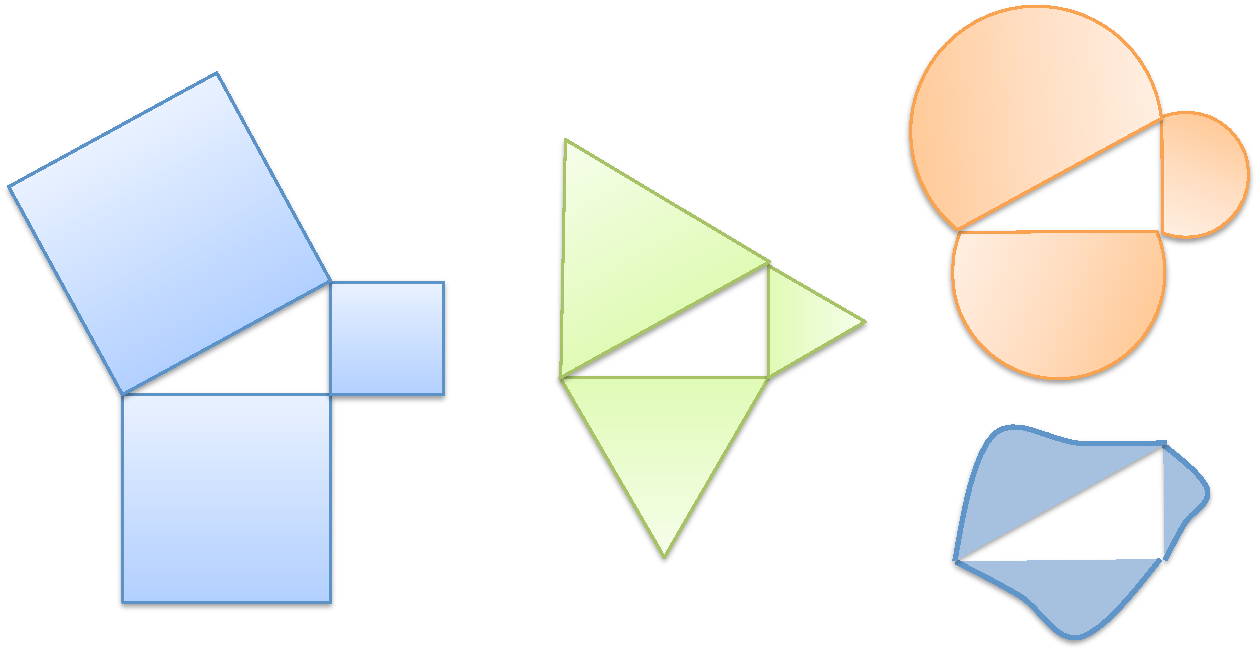
\includegraphics{./images/ch6/ggNew.pdf}}  
	\end{center}
\end{shaded}

{\bf 例:}$f(x)\in C[0,1]$且严格单调递增,$f(0)=0,f(1)=1$,已知
$\dint_0^1f(x)\d x=\df23$,求$\dint_0^1f^{-1}(y)\d y$

[提示]:作图易知
$$\dint_0^1f(x)\d x+\dint_0^1f^{-1}(y)\d y=1$$

\begin{center}
	\resizebox{!}{5cm}{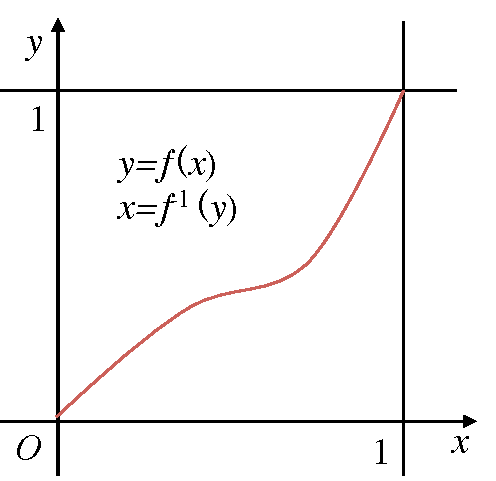
\includegraphics{./images/ch6/iff-1.pdf}}  
\end{center}

{\bf 例:}$a>1$,证明:$\dint_1^a\ln x\d x+\dint_0^{\ln a}e^y\d y=a\ln a$

[提示]:与上题同理。

\begin{thx}
	{\bf 定理:}$f(x)\in C[a,b]$严格单调增加,则
	$$\dint_a^bf(x)\d x+\dint_{f(a)}^{f(b)}f^{-1}(y)\d y=bf(b)-af(a)$$
\end{thx}

例如:
$$\dint_0^{\pi/2}\sin x\d x+\dint_0^1\arcsin x\d x=\df{\pi}2$$
\begin{center}
	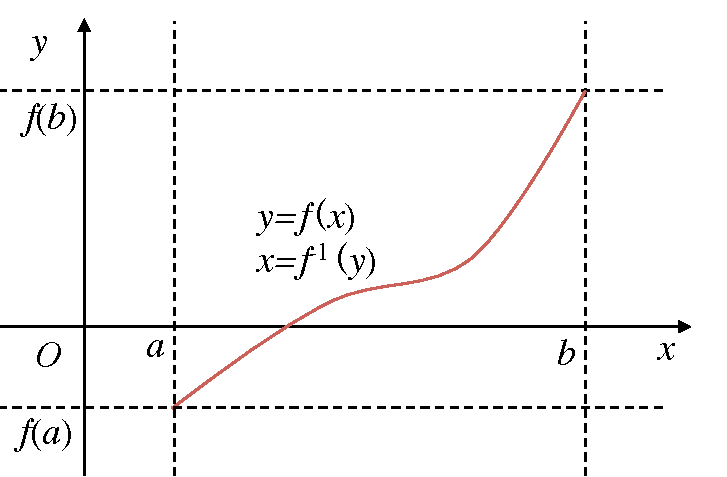
\includegraphics[width=5cm]{./images/ch6/iff-1ab.pdf}  
\end{center}

{\bf 例:}$f(x)\in C[0,+\infty)$且严格单调递增,$f(0)=0,a>0,b>0$,则
成立如下的Young{\it 不等式}
$$ab\leq\dint_0^af(x)\d x+\dint_0^bf^{-1}(y)\d y$$
\begin{center}
	\resizebox{!}{4cm}{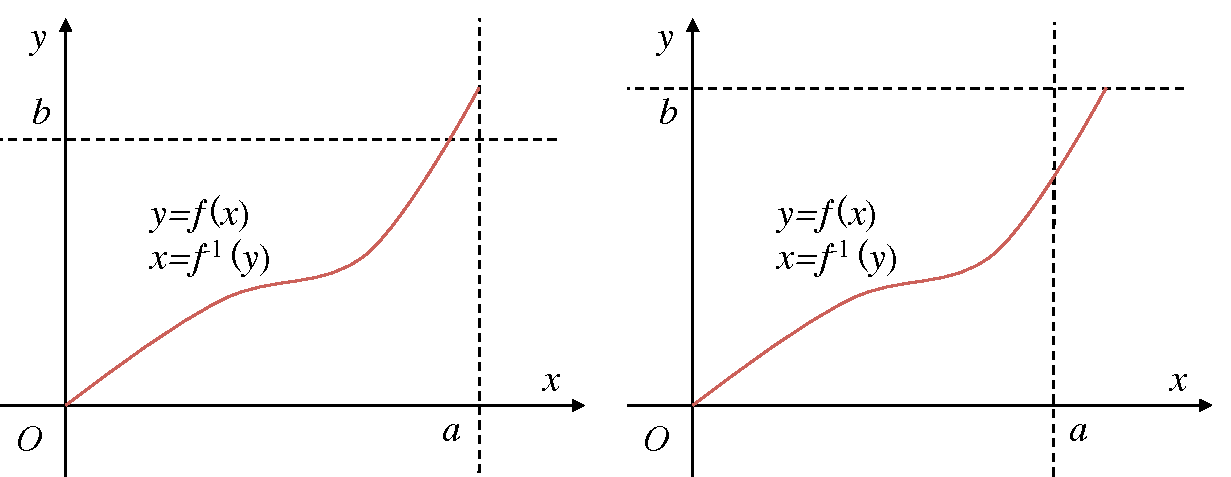
\includegraphics{./images/ch6/iff-ab.pdf}}  
\end{center}
利用该不等式,可以证明Minkowski{\it 不等式}:设$p>1,q>1,\df1p+\df1q=1$,则
$$ab\leq\df{a^p}p+\df{b^q}q$$
[提示]:令$f(x)=x^{p-1}$,则$x=y^{q-1}$(注意到$\df1{p-1}=q-1$)

{\bf 例:}计算$\dint_0^1\left(\sqrt[3]{1-x^7}-\sqrt[7]{1-x^3}\right)\d x$

[提示]:$y=\sqrt[3]{1-x^7}$和$x=\sqrt[7]{1-y^3}$互为反函数!

\begin{ext}
	{\bf 课后作业}
	
	\begin{enumerate}
	  \item 计算下列定积分
	  \begin{enumerate}[(1)]
	    \item $\dint_0^4e^{\sqrt x}\d x$
	    \item $\dint_{-\frac{\pi}2}^{\frac{\pi}2}(x^3+\sin^2x)\cos^2x\d x$
	    \item $\dint_0^{\frac{3\pi}4}\df{\d x}{1+\sin^2x}$
	    \item $\dint_0^{\frac{\pi}2}\df{\d x}{1+(\tan x)^{\sqrt 2}}$
	    \item $\dint_{\frac12}^{\frac32}\df{(1-x)\arcsin(1-x)}{\sqrt{2x-x^2}}\d x$
	    \item $\dint_{-\frac{\pi}4}^{\frac{\pi}4}e^{\frac x2}
	    \df{\cos x-\sin x}{\sqrt{\cos x}}\d x$
	    \item $\dint_{-2}^2\df{x+\sin x+|x|}{2+x^2}\d x$
	    \item $\dint_{\frac12}^{\frac32}\df{\d x}{\sqrt{|x^2-x|}}$
	  \end{enumerate}
	  \item 设$f(x),g(x)$在$[0,1]$上导函数连续,且$f(0)=0$,$f'(x)\geq0$,
	  $g'(x)\geq0$,证明:对任意$a\in[0,1]$,总有
	  $$\dint_0^ag(x)f'(x)\d x+\dint_0^1f(x)g'(x)\d x\geq f(a)g(1).$$
	  \item 设$f(x),g(x)$在$[a,b]$上连续,且满足
	  $$\dint_a^xf(t)\d t>\dint_a^xg(t)\d t,\;x\in[a,b),
	  \quad \dint_a^bf(x)\d x=\dint_a^bg(x)\d x,$$
	  证明:$\dint_a^bxf(x)\d x<\dint_a^bxg(x)\d x$。
	  \item 设$f(x)\in C[a,b]$且严格单调递增,证明:
	  $$(a+b)\dint_a^bf(x)\d x<2\dint_a^bxf(x)\d x.$$
	  \item 设$f(x)$是以$T$为周期的连续函数
	  \begin{enumerate}[(1)]
	    \item 证明:$\dint_0^xf(t)\d t$可以表示为一个以$T$
	    为周期的函数$g(x)$与$kx$之和,求此常数$k$;
	    \item 计算$\limx{\infty}\df1x\dint_0^xf(t)\d t$;
	    \item 设$[x]$为不超过$x$的最大整数,$g(x)=x-[x]$,计算
	    $\limx{\infty}\df1x\dint_0^xg(t)\d t$。
	  \end{enumerate}
	\end{enumerate}
\end{ext}

\section{反常积分}

定积分存在的条件:
$${I=\dint_a^bf(x)\d x}$$
\begin{enumerate} [(1)]
  \setlength{\itemindent}{1cm}
  \item {\it 有限区间:}$a,b\ne \infty$
  \item {\it 分段连续:}$f(x)$最多有限多个第一类间断点 
  \item {\it 必要条件:}$f(x)$有界
\end{enumerate}

从微积分基本公式出发,可以发现,即使以上的条件不能全部满足,
有时积分的值可能也是“可以计算出来的”。

\subsection{无穷限的反常积分}

\begin{thx}
	设函数$f(x)$在$[a,+\infty)$的任意有界子区间上可积,且
	极限$\lim\limits_{t\to+\infty}\dint_a^tf(x)\d x$
	存在,则称{\bf $f(x)$在$[a,+\infty)$上的无穷积分收敛},该极限称为
	{\bf $f(x)$在$[a,+\infty)$上的无穷积分},记为
	$$\dint_a^{+\infty}f(x)\d x.$$
\end{thx}
类似地,可以定义${\dint_{-\infty}^af(x)\d x}$和
${\dint_{-\infty}^{+\infty}f(x)\d x}$。

根据以上定义,可得无穷积分的Newton-Leibnitz公式:
  $$\dint_a^{+\infty}f(x)\d x=F(x)|_{a}^{+\infty}
  =\limx{+\infty}F(x)-F(a)$$
  
{\bf 例:}计算以下无穷积分
$$\dint_{-\infty}^{+\infty}\df{1}{1+x^2}\d x$$

\begin{center}
	\resizebox{!}{5cm}{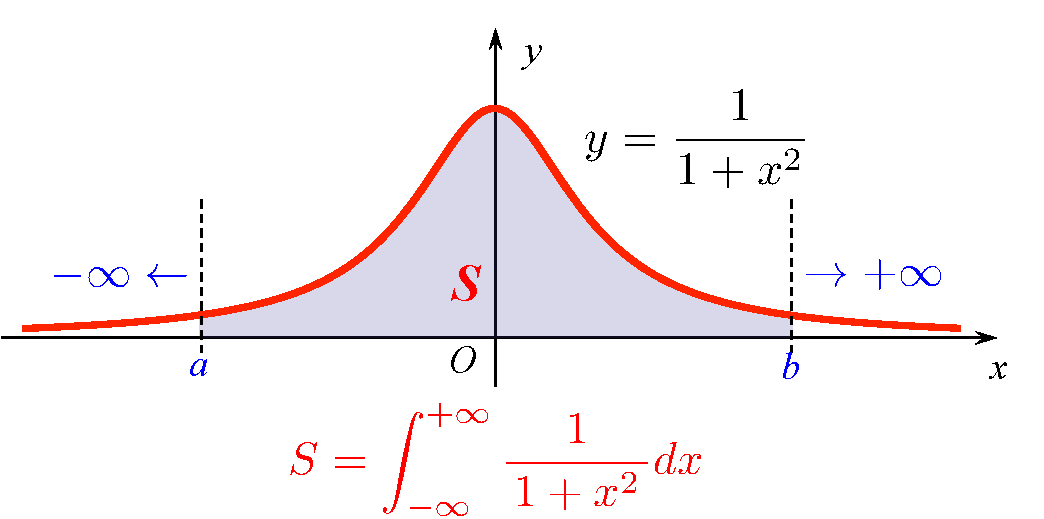
\includegraphics{./images/ch6/infint.pdf}}
\end{center}

{\bf 例:}
\begin{enumerate}[(1)]
  \setlength{\itemindent}{1cm}
  \item 讨论{\kaishu $p$-无穷积分}:$\dint_a^{+\infty}\df{\d x}{x^p},\;a>0, p>0$的敛散性; 
  \item 证明$$\dint_1^{n+1}\df 1{x^p}\d x<\sum\limits_{k=1}^n\df 1{k^p}
  <1+\dint_1^n\df{1}{x^p}\d x$$ 
  \item 根据以上结论判断{\kaishu $p$-级数}:$\sumn\df1{x^p}$的敛散性。
\end{enumerate}

[解]:(1)任取$t>a$。

若$p=1$,则
$$\dint_a^{+\infty}\df{\d x}{x^p}=\left.\ln|x|\right|_a^t=\ln\df ta,$$
显然,当$t\to+\infty$时,右端函数极限不存在,故此时$p$-无穷积分发散。

若$p\ne 1$,则
$$\dint_a^{+\infty}\df{\d x}{x^p}=\left.\df{x^{1-p}}{1-p}\right|_a^t
=\df{t^{1-p}-a^{1-p}}{1-p},$$
若$0<p<1$,当$t\to+\infty$时,右端函数极限不存在,故$p$-无穷积分发散;若$p<1$,
当$t\to+\infty$时,右端函数极限存在,故$p$-无穷积分收敛。

综上,
\begin{thx}
	{\bf $p$-无穷积分的敛散性:}$\dint_a^{+\infty}\df{\d x}{x^p}$当$0<p\leq 1$时发散;当$p>1$时收敛。	
\end{thx}

(2)
\begin{center}
	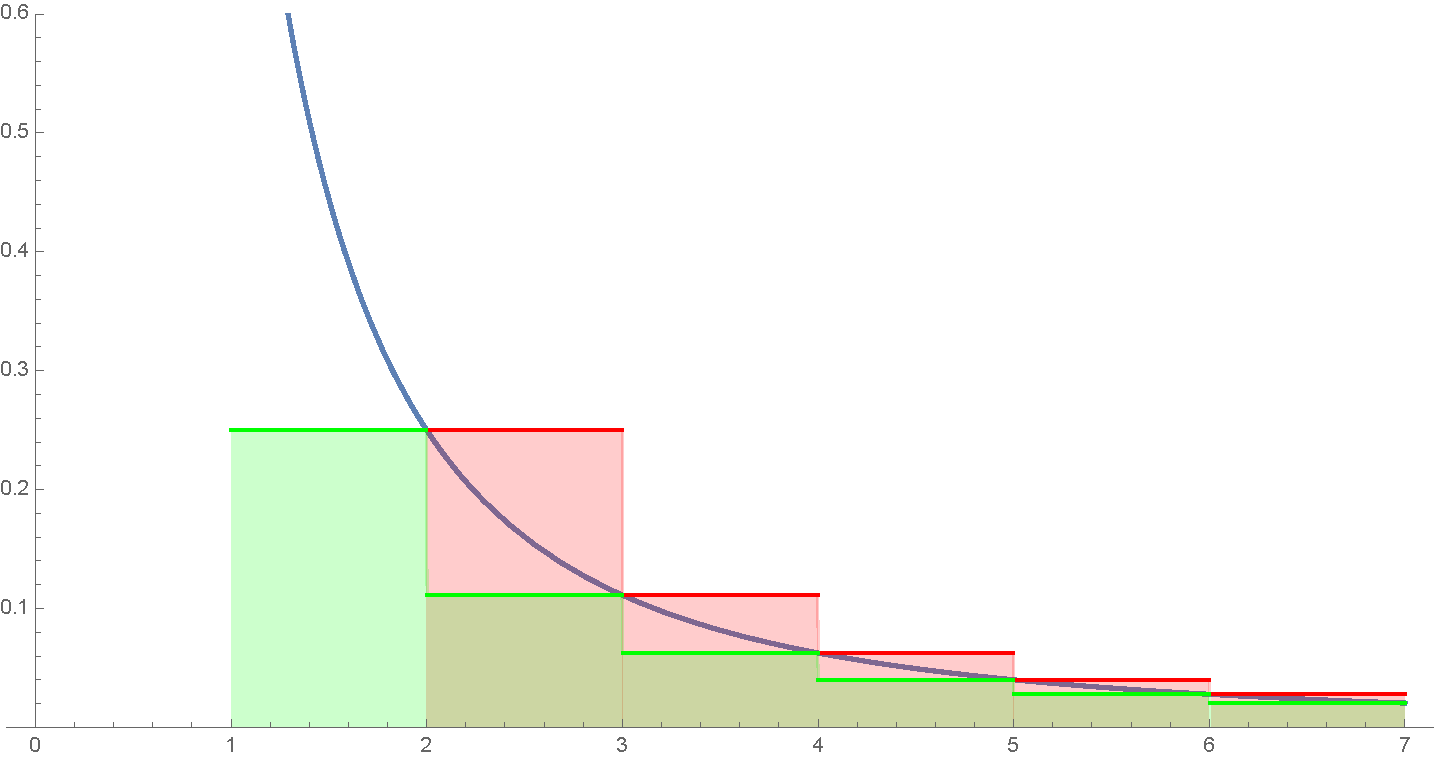
\includegraphics[width=7cm]{./images/ch5/xpVsSum.pdf}
\end{center}

如图,可知对任意$k>1$,总有
$$\dint_k^{k+1}\df{\d x}{x^p}<\df1{k^p}<\dint_{k-1}^k\df{\d x}{x^p},$$
两端对$k$从$1$至$n$求和(注意到$k=1$时,$\df1{k^p}=1$),即得
$$\dint_1^{n+1}\df 1{x^p}\d x=
\sum\limits_{k=1}^n\dint_k^{k+1}\df{\d x}{x^p}
<\sum\limits_{k=1}^n\df1{k^p}<
1+\sum\limits_{k=2}^n\dint_{k-1}^k\df{\d x}{x^p}
=1+\dint_1^n\df{1}{x^p}\d x.$$

(3)$p$-级数的收敛性等价于数列$\left\{\sum\limits_{k=1}^n
\df1{k^p}\right\}$的收敛性。根据(2)所得的不等式,可知$p$-级数与
$p$-积分同敛散。事实上,若$p>1$,则$p$-无穷积分收敛,设其值为$A$,则
由(2)中不等式和夹逼定理,可知此时$p$-级数收敛;反之,若$0<p\leq1$,
则由$p$-无穷积分发散,必有数列$\dint_1^{n+1}\df 1{x^p}\d x$发散至无穷,从而由
$\dint_1^{n+1}\df 1{x^p}\d x<\sum\limits_{k=1}^n\df1{k^p}$
可知$p$-级数必发散。\fin

参考本题的证明思路,可以证明如下的判别无穷级数收敛的方法:

\begin{thx}
	{\bf 无穷级数的积分判别法}:设$f(x)$在$[1,+\infty)$上非负单调递减,则
	无穷积分$\dint_1^{+\infty}f(x)\d x$与无穷级数$\sumn f(n)$同敛散。
\end{thx}

\begin{shaded}
	{\bf Gabriel's Horn Paradox}
	
	\begin{center}
		\resizebox{!}{5cm}{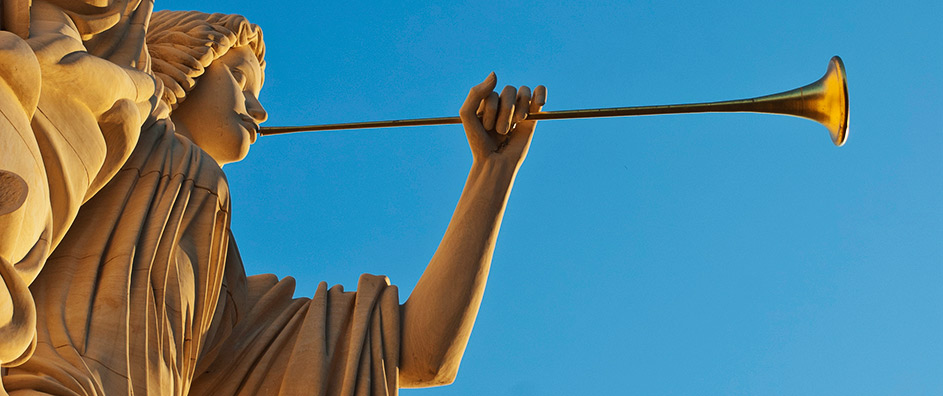
\includegraphics{./images/ch6/gabrielshorn.jpg}}
	\end{center}
	
	Gabriel是圣经故事中的大天使(Saint Gabriel the Archangel)之一
	(其他的还有Michael、Raphael等)
	,他吹奏一支长喇叭让魔鬼坠入地狱。关于长喇叭有如下的一个悖论
	(据说由Torricelli提出):设Gabriel喇叭由曲线$y=\df1x(x\geq 1)$
	围绕$x$轴旋转而成,证明:
	\begin{enumerate} [(1)]
  	  \setlength{\itemindent}{1cm}
	  \item 喇叭的体积是一个有限值
	  \item 喇叭的表面积为无穷大
	  \item 有前面的结论应该可以推论出这样的结果:Gabriel喇叭的内部可以被有限数量
	  的油漆填满,但同时,任何有限数量的漆都无法刷遍其内表面!该如何解释这个悖论呢?
	\end{enumerate}
	[提示]:
	(1)体积为
	$$V=\dint_1^{+\infty}\pi\left(\df1x\right)^2\d x=\pi$$
	(2)表面积
	$$A=2\pi\dint_1^{+\infty}y\sqrt{1+(y')^2}\d x=2\pi\dint_1^{+\infty}
	\df{\sqrt{x^4+1}\d x}{x^3}>2\pi\dint_1^{+\infty}\df1x\d x=+\infty$$
	(3)如果涂在表面上的漆的厚度可以是任意小,则任意有限数量的漆都可以刷遍整个喇叭。
	
	一个类似的论题:对于平面区域$D:x\geq0,y\in[0,1]$,给定一个单位质量的金箔,
	只要我们允许金珀铺的任意薄(厚度$h(x)=e^{-x}$),则可以将整个区域$D$铺满。
	
	{\bf 有限 vs. 无限:一个迷人的话题}
	
	关于类似这种{\kaishu 体积有限而表面积无限}的例子还有很多,比如下面的
	Serpinski三角和Menger六面体
	\begin{center}
		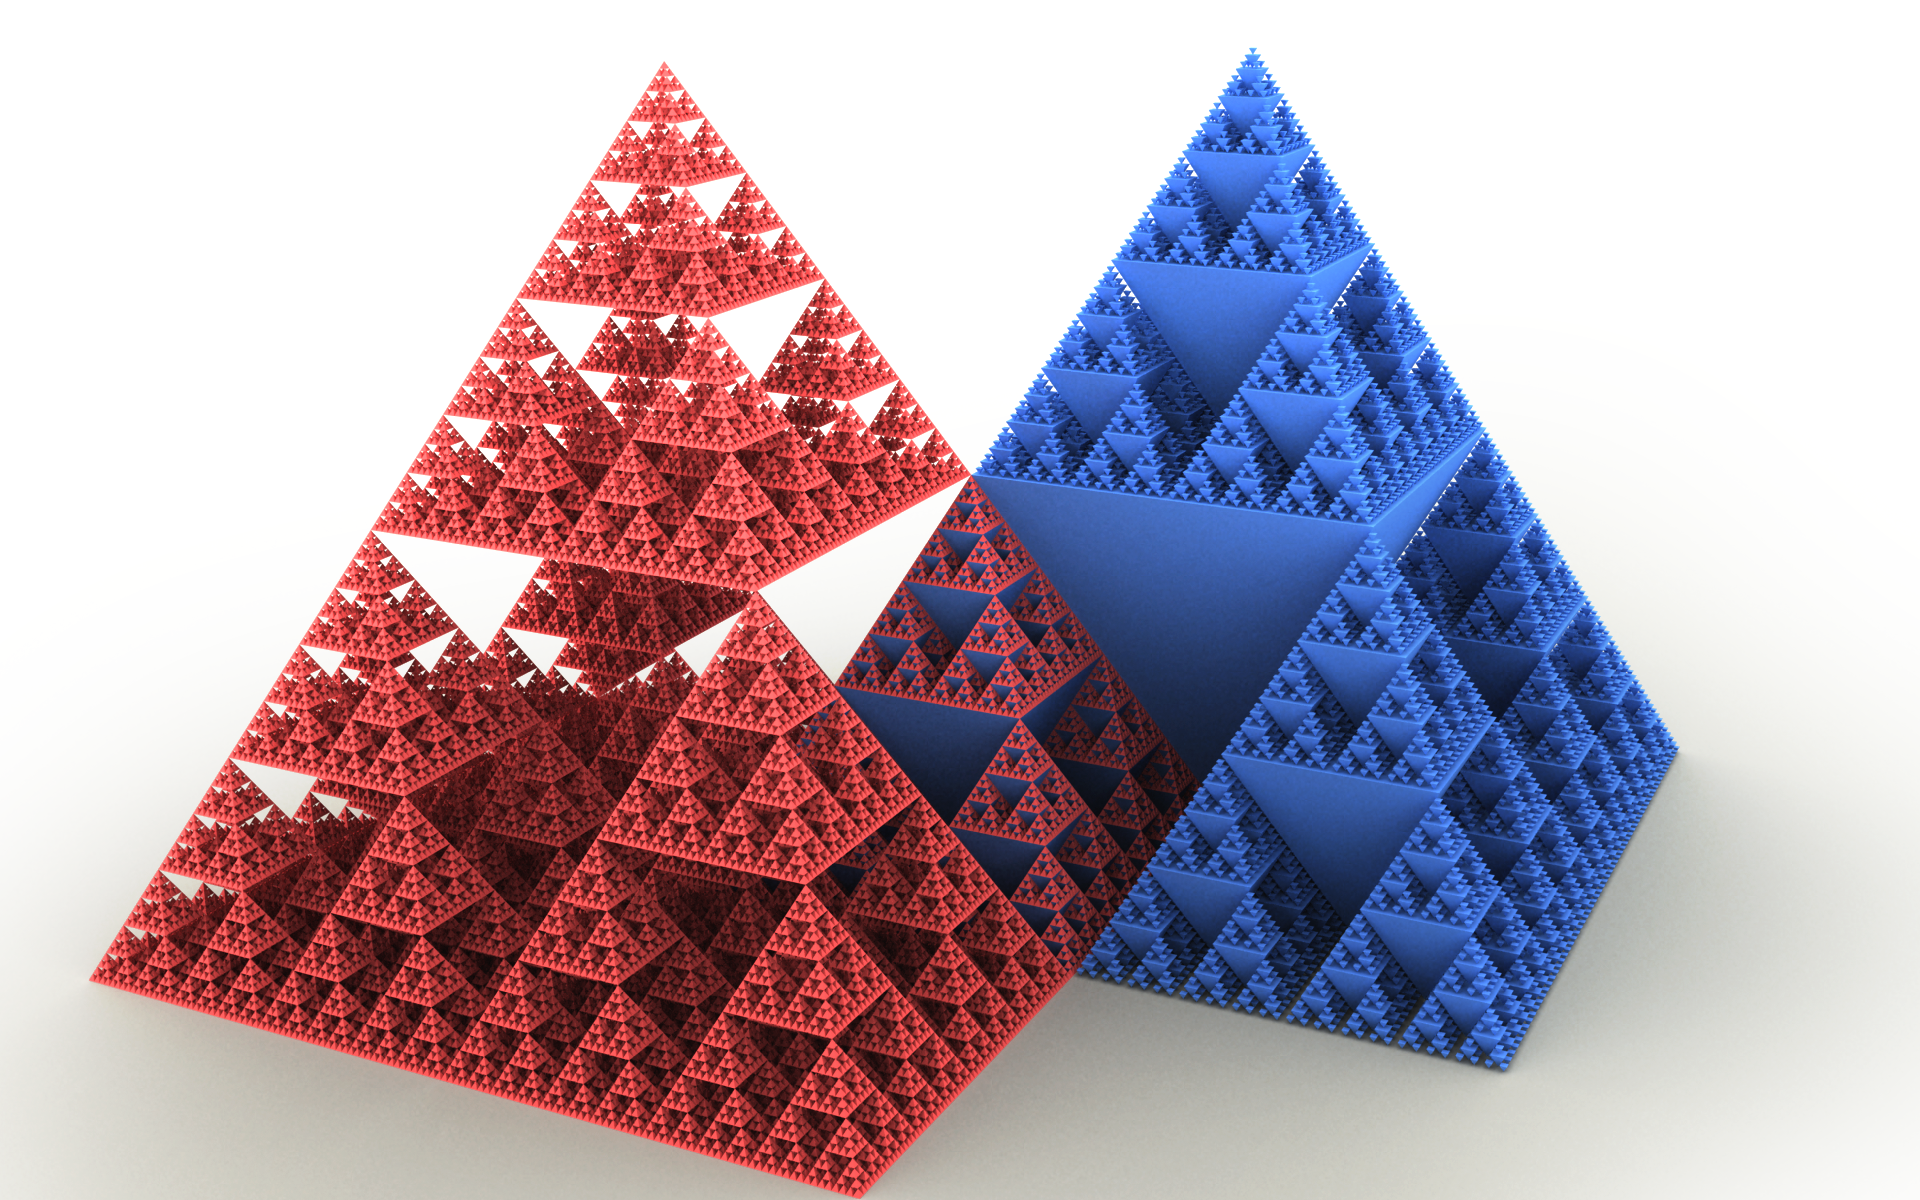
\includegraphics[height=4cm]{./images/ch5/sp-1.png}
		\includegraphics[height=4cm]{./images/ch5/ms-1.jpg}
	\end{center}
	此外,在平面上,{\kaishu 面积有限而边长无限}的例子也有很多,例如著名的
	Mandelbrot集和Julia集
	\begin{center}
		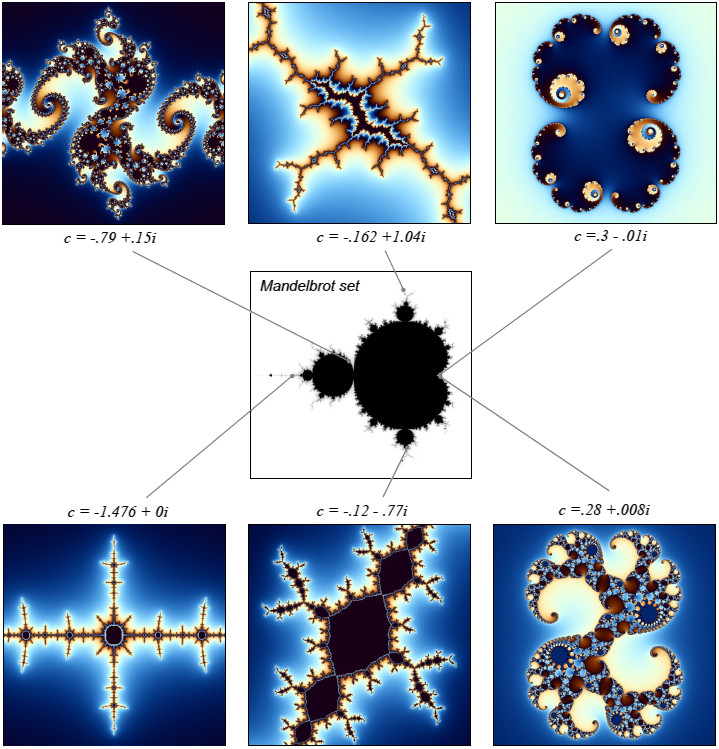
\includegraphics[height=8cm]{./images/ch5/mdbt.jpg}
		
		\includegraphics[height=4cm]{./images/ch5/jl-1.jpg}
		
\includegraphics[height=4cm]{./images/ch5/mdbt-2.png}
	\end{center}
	这些了不起的例子都属于当代数学里最“迷人”的分支之一——{\kaishu 分形几何},
	数学和艺术在这里相互交织,精彩绝伦。
\end{shaded}

\subsection{无界函数的反常积分}

无穷积分的几何意义相对于是求某个宽度为无穷(面积有限)的平面区域的面积,
类似地,如果某个平面区域的高度为无穷的,在一定条件下,其面积也可能是
有限的,这样的积分通常称为{\kaishu 瑕积分}。

\begin{thx}
	设函数$f(x)$在$(a,b]$上有定义,$\limx{a^+}f(x)=\infty$(此时称
	$x=a$是$f(x)$的{\bf 瑕点}),若极限$\limx{a^+}\dint_t^bf(x)\d x$
	存在,则称{\bf $f(x)$在$(a,b]$上的瑕积分收敛},极限的值称为
	{\bf $f(x)$在$(a,b]$上的瑕积分},记为$\dint_a^bf(x)\d x$
\end{thx}

显然,令$y=\df1{a-x}$或$y=\df1{x-a}$,总可以将一个瑕积分化为一个无穷积分。

{\bf 例:}计算
$$\dint_0^a\df{1}{\sqrt{a^2-x^2}}\d x,\;a>0$$

{\bf 例:}讨论{\kaishu $p$-瑕积分}:$\dint_0^a\df{\d x}{x^p}$的收敛性。

[解]:
$$\dint_0^a\df1{x^p}\d x
\xlongequal{y=\frac1x}\dint_{+\infty}^{\frac1a}y^p\d\df1y
=\dint_{\frac1a}^{+\infty}\df1{y^{2-p}}\d y.$$
由$p$-无穷积分的收敛性可知:$2-p>1$,也即$0<p<1$时,右端积分收敛,从而
$p$-瑕积分收敛;$2-p\leq 1$,也即$p\geq 1$时,右端积分发散,从而
$p$-瑕积分发散。\fin

\begin{thx}
	{\bf $p$-瑕积分的敛散性:}$\dint_0^a\df{\d x}{x^p}$当$p\geq 1$时发散,当
	$0<p<1$收敛。
\end{thx}

{\bf 例:}讨论瑕积分的收敛性
\begin{enumerate}[(1)]
  \setlength{\itemindent}{1cm}
  \item $\dint_{-1}^1\df{\d x}{x^2}$ 
  \item $\dint_{-1}^1\df{\d x}{x}$
\end{enumerate}

{\bf 例:}计算
$$\dint_0^{+\infty}\df{\d x}{\sqrt{x(x+1)^3}}$$

[解]:
$$
	\mbox{原式}
	=2\dint_0^{+\infty}\df{\d\sqrt x}{\sqrt{(x+1)^3}}
	\xlongequal{x=\tan^2t}2\dint_0^{\frac{\pi}2}\df{2\tan x\sec^2x\d x}
	{\sec^3x}
	=4\dint_0^{\frac{\pi}2}\sin x\d x=4.
$$
\fin

\begin{ext}
	{\bf 课后作业}	
	\begin{enumerate}
	  \item 计算下列积分
	  \begin{enumerate}[(1)]
	    \item $\dint_1^{+\infty}\df{\arctan x}{x^2}\d x$
% 	    \item $\dint_0^1\df1{\sqrt x}\dint_1^{\sqrt x}e^{-t^2}\d t\d x$
	    \item $\dint_2^{+\infty}\df{\d x}{(x+7)\sqrt{x-2}}$
	    \item (选作)$\dint_1^{+\infty}\df{\d x}{x\sqrt{1+2x^4+2x^8}}$
	    \item $\dint_{-1}^0\df{\ln(1+x)}{\sqrt[3]{1+x}}\d x$
	    \item $\dint_0^{+\infty}\df{\d x}{e^{x+1}+e^{1-x}}$
	  \end{enumerate}
	  \item 已知$\dint_0^{+\infty}\df{\sin x}x\d x=\df{\pi}2$,求
	  $\dint_0^{+\infty}\df{\sin^2x}{x^2}\d x$。
	\end{enumerate}
\end{ext}

\section{反常积分的审敛法与$\Gamma$函数}

由于有些反常积分无法直接计算(例如$\dint_0^{+\infty}e^{-x^2}\d x$),
要判断其是否收敛只能通过一些间接的手段来完成。

\subsection{无穷积分的审敛法}

以下以无穷积分为例讨论反常积分的一些审敛(判断收敛性)的方法。

% 首先,给出一个无穷积分收敛的必要条件:
% 
% \begin{thx}
% 	设$f(x)$在$x\geq a$上连续,且$\dint_a^{+\infty}f(x)\d x$收敛,
% 	则必有$f(+\infty)=0$。
% % \end{thx}
% 
% 这个结论我们不予证明。将其用于无穷积分的判敛,主要是通过验证被积函数不满足收敛
% 的必要条件,进而得出无穷积分不收敛的结论。

{\bf 例:}判断如下积分是否收敛:$\dint_1^{+\infty}\df{x^2}{x^2+1}\d x$。

[解]:显然$\limx{+\infty}\df{x^2}{x^2+1}=1\ne 0$,故由无穷积分收敛的必要
条件,该无穷积分发散。\fin

\begin{thx}
	{\bf 比较判别法:}设$f(x),g(x)$在$[a,+\infty)$上连续,且
	$$0\leq f(x)\leq g(x),\quad x\in[a,+\infty)$$ 
	\begin{enumerate}[(1)]
% 	  \setlength{\itemindent}{1cm}
	  \item
	  $\dint_a^{+\infty}g(x)\d x$收敛$\Rightarrow\dint_a^{+\infty}f(x)\d x$收敛 
	  \item $\dint_a^{+\infty}f(x)\d x$发散$\Rightarrow\dint_a^{+\infty}g(x)\d x$发散
	\end{enumerate}
\end{thx}

{\bf 例:}讨论以下无穷积分的敛散性
\begin{enumerate}[(1)]
  \setlength{\itemindent}{1cm}
  \item $\dint_2^{+\infty}\df{1+\sin x}{x^2}\d x$ 
  \item $\dint_1^{+\infty}\df{\d x}{\sqrt[3]{x^4+1}}$
\end{enumerate}

\begin{thx}
	{\bf 极限判别法:}设$f(x),g(x)$在$[a,+\infty)$上连续,$0\leq f(x)\leq g(x)$,且
	$$\limx{+\infty}\df{f(x)}{g(x)}=l$$ 
	\begin{enumerate}[(1)]
% 	  \setlength{\itemindent}{1cm}
	  \item $0<l<+\infty$,两个无穷积分同敛散 
	  \item
	  $l=0$,$\dint_a^{+\infty}g(x)\d x$收敛
	  $\Rightarrow\dint_a^{+\infty}f(x)\d x$收敛 
	  \item
	  $l=+\infty$,$\dint_a^{+\infty}f(x)\d x$发散
	  $\Rightarrow\dint_a^{+\infty}g(x)\d x$发散
	\end{enumerate}
\end{thx}

{\bf 例:}判定以下反常积分的收敛性
\begin{enumerate}[(1)]
  \setlength{\itemindent}{1cm}
  \item $\dint_1^{+\infty}\df{\d x}{x\sqrt{1+x^2}}$ 
  \item $\dint_1^{+\infty}\df{x^{3/2}}{1+x^2}\d x$ 
  \item $\dint_1^{+\infty}\df{\arctan x}{x}\d x$
\end{enumerate}

\begin{thx}
	{\bf 绝对收敛性:}设$f(x)$在$[a,+\infty)$上连续,
	若$\dint_a^{+\infty}|f(x)|\d x$收敛,则
	$\dint_a^{+\infty}f(x)\d x$收敛。
\end{thx}

{\bf 例:}讨论反常积分$\dint_0^{+\infty}e^{-ax}\sin bx\d x\;(a>0)$的敛散性。

{\bf 例:}判定下列积分的敛散性
\begin{enumerate}[(1)]
  \setlength{\itemindent}{1cm}
  \item $\dint_1^3\df{\d x}{\ln x}$ 
  \item $\dint_0^1\df{\d x}{\sqrt{(1-x^2)(1-k^2x^2)}}\;(k^2<1)$ 
  \item $\dint_0^1\df 1{\sqrt{x}}\sin\df 1x\d x$
\end{enumerate}

\subsection{$\Gamma$函数}

\begin{thx}
	$${\Gamma(s)=\dint_0^{+\infty}e^{-x}x^{s-1}\d x\;(s>0)}$$
\end{thx}

{\bf 例:}证明$\Gamma(s)=\dint_0^{+\infty}e^{-x}x^{s-1}\d x\;(s>0)$是收敛的。

[证]:显然$s=1$时,积分收敛。

当$s\ne1$时,$e^{-x}x^{s-1}<x^{s-1}\;(x>0)$,又$\dint_0^1x^{s-1}\d x=\df1s$,
故由比较判别法,$I_1=\dint_0^1e^{-x}x^{s-1}\d x$收敛。

由$\limx{+\infty}e^{-\frac x2}x^{s-1}=0$,存在$X>1$,对任意$x>X$,有
$e^{-\frac x2}x^{s-1}<1$,进而$e^{-x}x^{s-1}<e^{-\frac x2}$,又
$\dint_X^{+\infty}e^{-\frac x2}\d x=2e^{\frac X2}$,故由比较判别法,
$I_3=\dint_X^{+\infty}e^{-x}x^{s-1}\d x$收敛。

$I_2=\dint_1^Xe^{-x}x^{s-1}\d x$为定积分。

综上,$\Gamma(s)=I_1+I_2+I_3$收敛。\fin

\begin{thx}
	{\bf $\Gamma$函数的性质:}
	\begin{enumerate}
% 	  \setlength{\itemindent}{1cm}
	  \item $\Gamma(s+1)=s\Gamma(s)$ 
	  \item $\lim\limits_{s\to 0+}\Gamma(s)= +\infty$ 
	  \item $\Gamma(s)\Gamma(1-s)=\df{\pi}{\sin \pi s}\;(0<s<1)$ 
	  \item $2\dint_0^{+\infty}e^{-x^2}\d x=\Gamma\left(\df 12\right)=\sqrt{\pi}$
	\end{enumerate}
\end{thx}

\begin{ext}
	{\bf 课后作业}	
	\begin{enumerate}
	  \item 判定如下反常积分的敛散性
	  \begin{enumerate}[(1)]
	    \item $\dint_1^{+\infty}\df{x^2\d x}{(x+1)\sqrt[2]{x^3+1}}$
	    \item $\dint_1^2\df{\d x}{(\ln x)^4}$
	    \item $\dint_1^{+\infty}\sin\df1{x^2}\d x$
	    \item $\dint_1^2\df{\d x}{\sqrt{3x-x^2-2}}$
	    \item $\dint_2^{+\infty}\df{\cos x}{\ln x}\d x$
	  \end{enumerate}
	  \item 设反常积分$\dint_1^{+\infty}f^2(x)\d x$收敛,证明反常积分
	  $\dint_1^{+\infty}\df{f(x)}x\d x$绝对收敛。
	  \item 利用$\Gamma$函数的性质证明{\kaishu Legendre倍量公式}:
	  $$\sqrt{\pi}\Gamma(2n)=2^{2n-1}\Gamma(n)\Gamma\left(n+\df12\right).$$
	\end{enumerate}
\end{ext}

\visibletrue

\ifvisible

\newpage

\section*{作业参考解答}
% \addcontentsline{toc}{section}{作业参考解答}

\begin{center}
	\bf 5.1 定积分的概念与性质
\end{center}

\bigskip

1.设$f(x)$在$[a,b]$上非负,当$x\in(a,b)$内$f''(x)>0,f'(x)<0$,
$I_1=\df{b-a}2[f(b)+f(a)]$,$I_2=\dint_a^bf(x)\d x$,$I_3=(b-a)f(b)$,
试比较$I_1,I_2,I_3$的大小。

[解]:$f'(x)<0$,故对任意$x\in(a,b)$,均有$f(a)>f(x)>f(b)$,从而
$$(b-a)f(a)>\dint_a^bf(x)\d x>(b-a)f(b),$$
由此可知$I_2>I_3$。

令$L(x)=f(a)+\df{f(b)-f(a)}{b-a}(x-a)$,
由$f''(x)>0$,可知对任意$x\in(a,b)$,均有$f(x)<L(x)$,进而
由定积分的保号性,可得
$$\dint_a^bf(x)\d x<\dint_a^bL(x)\d x=\df{b-a}2[f(b)+f(a)],$$
由此可得$I_2<I_1$。

综上,$I_1>I_2>I_3$。\fin

\bs

2.设$f(x)\in C[0,1]$,证明:$\dint_0^1f^2(x)\d x\geq
\left(\dint_0^1f(x)\d x\right)^2$.

[提示]:令$g(x)=1$,参考Schwarz不等式的证明方法即可。

\bs

3.设$f(x)\in C[a,b]$,$g(x)>0$,证明:存在$\xi\in[a,b]$,使得
$$\dint_a^bf(x)g(x)\d x=f(\xi)\dint_a^bg(x)\d x.$$

[证]:由$f(x)\in C[a,b]$,可设$m,M$分别为$f(x)$在$[a,b]$上的
最小和最大值,进而可知
$$m\dint_a^bg(x)\d x\leq \dint_a^bf(x)g(x)\d x\leq M\dint_a^bg(x)\d x,$$
从而
$$m\leq\df{\dint_a^bf(x)g(x)\d x}{\dint_a^bg(x)\d x}\leq M,$$
从而由连续函数的介值定理可知,必存在$\xi\in[a,b]$,使得
$$f(\xi)=\df{\dint_a^bf(x)g(x)\d x}{\dint_a^bg(x)\d x}.$$
即证。\fin

\bs

4.已知$f(x)$在$[0,\pi]$上连续,$(0,\pi)$内可导,且$f(0)=
\dint_0^{\pi}f(x)\sin x\d x=0$,证明:存在$\xi\in(0,\pi)$,
使得$f'(\xi)=0$。

[证]:由$\dint_0^{\pi}f(x)\sin x\d x=0$,可知必存在$\eta\in(0,\pi)$,
使得$f(\eta)\sin\eta=0$,注意到$x\in(0,\pi)$时,$\sin x>0$,故必有
$f(\eta)=0$。至此,可以验证$f(x)$在$[0,\eta]$上满足Rolle定理条件,
进而可知必存在$\xi\in(0,\eta)\subset (0,\pi)$,使得$f'(\xi)=0$。\fin

5.设$f(x)$在$[0,1]$上连续,在$(0,1)$内可导,且$f(0)\cdot f(1)>0$,
$f(1)+\dint_0^1f(x)\d x=0$,证明:存在$\xi\in(0,1)$,使得
$f'(\xi)=\xi f(\xi)$。

[证]:不妨设$f(1)>0$,则$\dint_0^1f(x)\d x<0$,从而可知,存在$\eta_1\in(0,1)$,
使得$f(\eta_1)<0$。进而由连续函数的介值定理,可知存在$\eta\in(0,\eta_1)$,
使得$f(\eta)=0$。

令$F(x)=e^{-\frac{x^2}2}f(x)$,可以验证$F(x)$在$[0,\eta]$上满足
Rolle定理条件,从而可知必存在$\xi\in(0,\eta)\subset(0,1)$,使得
$$F'(\xi)=e^{-\frac{\xi^2}2}[f'(\xi)-\xi f(\xi)]=0,$$
因为$e^{-\frac{\xi^2}2}\ne0$,故必有$f'(\xi)-\xi f(\xi)=0$,即证。\fin

\begin{center}
	\bf 5.2 微积分基本公式
\end{center}

1.计算下列定积分

(1)$\dint_{-1}^2[x]\max\{1,e^{-x}\}\d x$,其中$[x]$表示不超过$x$的最大整数;

[解]:
$$
	\dint_{-1}^2[x]\max\{1,e^{-x}\}\d x
	=-\dint_{-1}^0e^{-x}\d x+\dint_1^2\d x
	=2-e
$$

(2)$\dint_0^{\pi}x\sqrt{\cos^2x-\cos^4x}\d x$

[解]:
\begin{align*}
	&\dint_0^{\pi}x\sqrt{\cos^2x-\cos^4x}\d x
	=\dint_0^{\pi}x|\sin x||\cos x|\d x\\
	&=\dint_0^{\frac{\pi}2}x\sin x\cos x\d x
	-\dint_{\frac{\pi}2}^{\pi}x\sin x\cos x\d x\\
	&=\df12\left(\dint_0^{\frac{\pi}2}x\sin2x\d x
	-\dint_{\frac{\pi}2}^{\pi}x\sin2x\d x\right)\\
	&=-\df14\left(\dint_0^{\frac{\pi}2}x\d\cos2x
	-\dint_{\frac{\pi}2}^{\pi}x\d\cos2x\right)\\
	&=-\df14\left(x\cos2x|_0^{\frac{\pi}2}
	-x\cos2x|_{\frac{\pi}2}^{\pi}\right)+
	\df14\left(\dint_0^{\frac{\pi}2}\cos2x\d x
	-\dint_{\frac{\pi}2}^{\pi}\cos2x\d x\right)\\
	&=-\df14\left(-\df{\pi}2-\pi-\df{\pi}2\right)
	+\df18\left(\sin2x|_0^{\frac{\pi}2}
	-\sin2x|_{\frac{\pi}2}^{\pi}\right)=\df{\pi}2.
\end{align*}

(3)设$f(x)=\left\{\begin{array}{ll}
	1+x^2, & x\leq0,\\ e^{-x}, & x>0
\end{array}\right.$,求$\dint_1^3f(x-2)\d x$

[解]:
\begin{align*}
	\dint_1^3f(x-2)\d x
	&=\dint_{-1}^1f(x)\d x
	=\dint_{-1}^0(1+x^2)\d x+\dint_0^1e^{-x}\d x\\
	&=1+\df13-e^{-1}+1=\df73-e^{-1}.
\end{align*}
\fin

\bs

2.已知$f(x)$连续,且$\dint_0^xtf(x-t)\d t=1-\cos x$,
求$\dint_0^{\frac{\pi}2}f(x)\d x$。

[解]:令$u=x-t$,则
$$\dint_0^xtf(x-t)\d t=\dint_x^0(x-u)f(u)\d(x-u)
=\dint_0^x(x-u)f(u)\d u=x\dint_0^xf(u)\d u-\dint_0^xuf(u)\d u.$$
故对已知等式两边关于$x$连续求导可得
$$\dint_0^xf(u)\d u=\sin x
\quad\Rightarrow\quad
f(x)=\cos x,$$
于是可得
$$\dint_0^{\frac{\pi}2}f(x)\d x=\dint_0^{\frac{\pi}2}\cos\d x=1.$$
\fin

\bs

3.计算下列函数的导函数

(1)$f(x)=\dint_0^xtg(x^2-t^2)\d t$,其中$g(x)$为连续函数;

[解]:令$u=x^2-t^2$,则
\begin{align*}
	f(x)&=\df12\dint_0^xg(x^2-t^2)\d t^2\\
	&=\df12\dint_{x^2}^0g(u)\d(x^2-u)
	=\df12\dint_0^{x^2}g(u)\d u,
\end{align*}
于是
$$f'(x)=\df12g(x^2)2x=xg(x^2).$$

(2)$f(x)=\dint_0^x\sin(x-t)^2\d t$。

[解]:令$u=x-t$,则
$$f(x)=\dint_x^0\sin u^2\d(x-u)=\dint_0^x\sin u^2\d u,$$
故
$$f'(x)=\sin x^2.$$
\fin

\bs

4.设曲线$y=f(x)$与$y=\dint_0^{\arctan x}e^{-t^2}\d t$在原点处
相切,求$\limn nf\left(\df2n\right)$。

[解]:
\begin{align*}
	\limn nf\left(\df2n\right)
	&=2\limn\df{f\left(\df2n\right)}{\df2n}
	=2\limx0\df{f(x)}x\\
	&=2\limx0f'(x)=2f'(0)=2y'(0)\\
	&=2e^{-\arctan^2 x}\left.\df1{1+x^2}\right|_{x=0}=2.
\end{align*}
\fin

\bs

5.求$a$的值,使得$\limx{\infty}\left(\df{1+x}x\right)^{ax+1}
=\dint_{-\infty}^ate^t\d t$。

[解]:
\begin{align*}
	\mbox{左边}&=\limx{\infty}\left(1+\df1x\right)^{x.\cdot\frac{ax+1}x}
	=e^a\\
	\mbox{右边}&=\dint_{-\infty}^at\d e^t
	=\left.te^t\right|_{-\infty}^a-\dint_{-\infty}^ae^t\d t
	=(a-1)e^a.
\end{align*}
由此易知$a=2$。\fin

\bs

6.计算如下极限

(1)$\limn\sum\limits_{k=1}^n\sqrt{\df{n+k}{n^3}}$

[解]
$$
\mbox{原式}=\limn\sum\limits_{k=1}^n\df1n\sqrt{1+\df kn}
=\dint_0^1\sqrt{1+x}\d x
=\df23(1+x)^{\frac32}|_0^1=\df23(2\sqrt2-1).
$$

(2)$\limn\sum\limits_{k=1}^n\df{n^2-k^2}{n^3}$

[解]:
$$
\mbox{原式}=\limn\sum\limits_{k=1}^n\df1n\left[1-\left(\df kn\right)^2\right]
=\dint_0^1(1-x^2)\d x=\df23.
$$

(3)$\limx{+\infty}\df{\dint_0^x(\arctan t)^2\d t}{\sqrt{x^2+1}}$

[解]:
$$
\mbox{原式}=\limx{+\infty}\df{\dint_0^x(\arctan t)^2\d t}{x}
=\limx{+\infty}(\arctan x)^2=\df{\pi^2}4.
$$
\fin

\begin{center}
	\bf 5.3 定积分的计算-换元法和分部积分法
\end{center}

\bs

1.计算下列定积分

(1)$\dint_0^4e^{\sqrt x}\d x$

[解]:
$$\mbox{原式}\xlongequal{t=\sqrt x}
\dint_0^2e^t2t\d t=2te^t|_0^2-2\dint_0^2e^t\d t
=2e^2+2.$$

(2)$\dint_{-\frac{\pi}2}^{\frac{\pi}2}(x^3+\sin^2x)\cos^2x\d x$

[解]:由对称区间上定积分的性质,
$\dint_{-\frac{\pi}2}^{\frac{\pi}2}x^3\cos^2x\d x=0$,
又注意到$\dint_{-\frac{\pi}2}^{\frac{\pi}2}\cos4x\d x=0$
故
\begin{align*}
	\mbox{原式}
	&=\dint_{-\frac{\pi}2}^{\frac{\pi}2}\sin^2x\cos^2x\d x
	=\df14\dint_{-\frac{\pi}2}^{\frac{\pi}2}\sin^22x\d x\\
	&=\df12\dint_{0}^{\frac{\pi}2}\df{1-\cos 4x}2\d x
	=\df{\pi}{8}.
\end{align*}

(3)$\dint_0^{\frac{3\pi}4}\df{\d x}{1+\sin^2x}$

[解]:
\begin{align*}
	\mbox{原式}&=\dint_0^{\frac{3\pi}4}\df{\csc^2x\d x}{\csc^2x+1}
	=-\dint_0^{\frac{3\pi}4}\df{\d\cot x}{\cot^2x+2}
	=-\df1{\sqrt2}\dint_0^{\frac{3\pi}4}\df{\d\frac{\cot x}{\sqrt2}}
	{\left(\frac{\cot x}{\sqrt2}\right)^2+1}\\
	&=-\left.\df1{\sqrt2}\arctan\df{\cot x}{\sqrt2}\right|_0^{\frac{3\pi}4}
	=\df1{\sqrt3}\arctan\df1{\sqrt2}.
\end{align*}

(4)$\dint_0^{\frac{\pi}2}\df{\d x}{1+(\tan x)^{\sqrt 2}}$

[解]:由对称性
\begin{align*}
	\mbox{原式}&=\dint_0^{\frac{\pi}2}\df{(\cos x)^{\sqrt 2}\d x}
	{(\cos x)^{\sqrt 2}+(\sin x)^{\sqrt 2}}
	=\dint_0^{\frac{\pi}2}\df{(\sin x)^{\sqrt 2}\d x}
	{(\cos x)^{\sqrt 2}+(\sin x)^{\sqrt 2}}\\
	&=\df12\dint_0^{\frac{\pi}2}\df{(\cos x)^{\sqrt 2}+(\sin x)^{\sqrt 2}}
	{(\cos x)^{\sqrt 2}+(\sin x)^{\sqrt 2}}\d x
	=\df12\dint_0^{\frac{\pi}2}\d x=\df{\pi}4.
\end{align*}

(5)$\dint_{\frac12}^{\frac32}\df{(1-x)\arcsin(1-x)}{\sqrt{2x-x^2}}\d x$

[解]:注意到
$$\dint_{\frac12}^1\df{(1-x)\arcsin(1-x)}{\sqrt{2x-x^2}}\d x
\xlongequal{y=2-x}\dint_1^{\frac32}\df{(1-y)\arcsin(1-y)}
{\sqrt{2y-y^2}}\d y,$$
故
\begin{align*}
	\mbox{原式}
	&=2\dint_{\frac12}^1\df{(1-x)\arcsin(1-x)}{\sqrt{2x-x^2}}\d x
	=2\dint_{\frac12}^1\df{(1-x)\arcsin(1-x)}{\sqrt{1-(1-x)^2}}\d x\\
	&\xlongequal{t=1-x}2\dint_0^{\frac12}\df{t\arcsin t}{\sqrt{1-t^2}}\d t
	=-2\dint_0^{\frac12}\arcsin t\d{\sqrt{1-t^2}}\\
	&=-2\left.\sqrt{1-t^2}\arcsin t\right|_0^{\frac12}
	+2\dint_0^{\frac12}\d t
	=-\df{\sqrt3\pi}6+1.
\end{align*}

(6)$\dint_{-\frac{\pi}4}^{\frac{\pi}4}e^{\frac x2}
\df{\cos x-\sin x}{\sqrt{\cos x}}\d x$

[解]:
\begin{align*}
	\mbox{原式}
	&=\dint_{-\frac{\pi}4}^{\frac{\pi}4}e^{\frac x2}\sqrt{\cos x}\d x
	+2\dint_{-\frac{\pi}4}^{\frac{\pi}4}e^{\frac x2}\d\sqrt{\cos x}\\
	&=\dint_{-\frac{\pi}4}^{\frac{\pi}4}e^{\frac x2}\sqrt{\cos x}\d x
	+2\left.e^{\frac x2}\sqrt{\cos x}\right|_{-\frac{\pi}4}^{\frac{\pi}4}
	-\dint_{-\frac{\pi}4}^{\frac{\pi}4}e^{\frac x2}\sqrt{\cos x}\d x\\
	&=\sqrt[4]8\left(e^{\frac{\pi}8}-e^{-\frac{\pi}8}\right).
\end{align*}

(7)$\dint_{-2}^2\df{x+\sin x+|x|}{2+x^2}\d x$

[解]:
\begin{align*}
	\mbox{原式}
	&=\dint_{-2}^2\df{|x|}{2+x^2}\d x
	=2\dint_0^2\df{x}{2+x^2}\d x
	=\dint_0^2\df{\d x^2}{2+x^2}
	=\left.\ln(2+x^2)\right|_0^2=\ln3.
\end{align*}

(8)$\dint_{\frac12}^{\frac32}\df{\d x}{\sqrt{|x^2-x|}}$

[解]:
\begin{align*}
	\mbox{原式}
	&=\dint_{\frac12}^1\df{\d x}{\sqrt{x(1-x)}}
	+\dint_1^{\frac32}\df{\d x}{\sqrt{x(x-1)}}\\
	&=2\dint_{\frac12}^1\df{\d\sqrt x}{\sqrt{1-(\sqrt x)^2}}
	+2\dint_1^{\frac32}\df{\d\sqrt x}{\sqrt{(\sqrt x)^2-1}}\\
	&=2\left.\arcsin\sqrt x\right|_{\frac12}^1
	+2\dint_0^{\arccos\sqrt{\frac23}}\df{\d\sec t}{\sqrt{\sec^2t-1}}\\
	&=\df{\pi}8+2\dint_0^{\arccos\sqrt{\frac23}}\sec t\d t\\
	&=\df{\pi}8+2\ln\left|\sec t+\tan t\right|_0^{\arccos\sqrt{\frac23}}
	=\df{\pi}2+\ln(2+\sqrt3).
\end{align*}

\bs

2.设$f(x),g(x)$在$[0,1]$上导函数连续,且$f(0)=0$,$f'(x)\geq0$,
$g'(x)\geq0$,证明:对任意$a\in[0,1]$,总有
$$\dint_0^ag(x)f'(x)\d x+\dint_0^1f(x)g'(x)\d x\geq f(a)g(1).$$

[证]:由$f(0)=0$,
$$\dint_0^1f(x)g'(x)\d x=\dint_0^1f(x)\d g(x)
=\left.f(x)g(x)\right|_0^1-\dint_0^1g(x)\d f(x)
=f(1)g(1)-\dint_0^1g(x)f'(x)\d x.$$
故待证不等式左端即为$f(1)g(1)+\dint_1^ag(x)f'(x)\d x$,令
$$F(a)=\dint_1^ag(x)f'(x)\d x+f(1)g(1)-f(a)g(1),$$
则$F'(a)=f'(a)[g(a)-g(1)]$。已知$g'(x)\geq0$,故
$g(a)-g(1)\leq 0$,又$f'(x)\geq0$,故$F'(a)\leq0$,
也即$F(a)$在$[0,1]$上单调递减。注意到$F(1)=0$,从而可知
$F(a)\geq 0$,即证。\fin

\bs

3.设$f(x),g(x)$在$[a,b]$上连续,且满足
$$\dint_a^xf(t)\d t>\dint_a^xg(t)\d t,\;x\in[a,b),
\quad \dint_a^bf(x)\d x=\dint_a^bg(x)\d x,$$
证明:$\dint_a^bxf(x)\d x<\dint_a^bxg(x)\d x$。

[证]:记$H(x)=\dint_a^x[f(t)-g(t)]\d t$,则由已知可得
$H(x)\geq 0$,$H(b)=H(a)=0$,于是
\begin{align*}
	\dint_a^bx[f(x)-g(x)]\d x
	&=\dint_a^bx\d H(x)
	=\left.xH(x)\right|_a^b-\dint_a^bH(x)\d x
	=-\dint_a^bH(x)\d x\leq 0,
\end{align*}
即证。\fin

4.设$f(x)\in C[a,b]$且严格单调递增,证明:
$$(a+b)\dint_a^bf(x)\d x<2\dint_a^bxf(x)\d x.$$

[证法一]:注意到
$$\dint_a^b\left(x-\df{a+b}2\right)f\left(\df{a+b}2\right)\d x=0,$$
故
\begin{align*}
	\dint_a^b\left(x-\df{a+b}2\right)f(x)\d x
	&=\dint_a^b\left(x-\df{a+b}2\right)\left[f(x)
	-f\left(\df{a+b}2\right)\right]\d x,
\end{align*}
由于$f(x)$在$[a,b]$上严格单调递增,故对任意$x\in(a,b)$,均有
$$\left(x-\df{a+b}2\right)\left[f(x)
-f\left(\df{a+b}2\right)\right]>0,$$
从而可知
$$\dint_a^b\left(x-\df{a+b}2\right)f(x)\d x>0,$$
即证。\fin

[证法二]:
\begin{align*}
	\dint_{\frac{a+b}2}^b\left(x-\df{a+b}2\right)f(x)\d x
	&\xlongequal{y=a+b-x}\dint_{\frac{a+b}2}^a
	\left(\df{a+b}2-y\right)f(a+b-y)\d (a+b-y)\\
	&=-\dint_a^{\frac{a+b}2}
	\left(y-\df{a+b}2\right)f(a+b-y)\d y
\end{align*}
故
\begin{align*}
	\dint_a^b\left(x-\df{a+b}2\right)f(x)\d x
	&=\left(\dint_a^{\frac{a+b}2}+\dint_{\frac{a+b}2}^b\right)
	\left(x-\df{a+b}2\right)f(x)\d x\\
	&=\dint_a^{\frac{a+b}2}\left(x-\df{a+b}2\right)
	[f(x)-f(a+b-x)]\d x,
\end{align*}
注意到当$x\in\left(a,\df{a+b}2\right)$时,总有$x-\df{a+b}2<0$,
$f(x)-f(a+b-x)<0$,故$\left(x-\df{a+b}2\right)[f(x)-f(a+b-x)]>0$,
进而可知以上右侧的积分必大于零,即证。\fin

[证法三]:令
$$F(x)=(a+x)\dint_a^xf(t)\d t-2\dint_a^xtf(t)\d t,$$
则
$$F'(x)=\dint_a^x[f(t)-f(x)]\d t,$$
由于$f(x)$严格单调递增,故总有$f(t)-f(x)<0$,进而$F'(x)<0$,
又$F(a)=0$,从而可知$F(b)<0$,即证。\fin

5.设$f(x)$是以$T$为周期的连续函数
  \begin{enumerate}[(1)]
    \setlength{\itemindent}{1cm}
    \item 证明:$\dint_0^xf(t)\d t$可以表示为一个以$T$
    为周期的函数$g(x)$与$kx$之和,求此常数$k$;
    \item 计算$\limx{\infty}\df1x\dint_0^xf(t)\d t$;
    \item 设$[x]$为不超过$x$的最大整数,$g(x)=x-[x]$,计算
    $\limx{\infty}\df1x\dint_0^xg(t)\d t$。
  \end{enumerate}

[解]:(1)记$k=\df1T\dint_0^Tf(x)\d x$,令$g(x)=\dint_0^xf(t)\d t-kx$,
则对任意$x$,有
\begin{align*}
	g(x+T)
	&=\dint_0^{x+T}f(t)\d t-k(x+T)
	=\dint_0^xf(t)\d t-kx+\dint_x^{x+T}f(t)\d t-kT\\
	&=g(x)+\dint_0^{T}f(t)\d t-kT=g(x),
\end{align*}
也即$g(x)$是以$T$为周期的函数,即证。

(2)显然$g(x)$是一个连续的周期函数,故必有界,从而可知$\limx{\infty}\df{g(x)}x=0$,
于是
$$\limx{\infty}\df1x\dint_0^xf(t)\d t=\limx{\infty}\df{g(x)+kx}x=k
=\df1T\dint_0^Tf(x)\d x.$$

(3)$g(x)$是以$1$为周期的函数,且$\dint_0^1(x-[x])\d x=\df12$,故由(2)的结论,
可知$\limx{\infty}\df1x\dint_0^xg(t)\d t=\df12$。\fin

\begin{center}
	\bf 5.4 反常积分
\end{center}

1.计算下列积分

(1)$\dint_1^{+\infty}\df{\arctan x}{x^2}\d x$

[解]:
\begin{align*}
	\mbox{原式}
	&=-\dint_1^{+\infty}\arctan x\d\df1x
	=-\left.\df{\arctan x}x\right|_1^{+\infty}
	+\dint_1^{+\infty}\df1x\d\arctan x\\
	&=\df{\pi}4+\dint_1^{+\infty}\df1{x(1+x^2)}\d x
	=\df{\pi}4+\df12\dint_1^{+\infty}\left(\df1{x^2}-\df1{1+x^2}\right)\d x^2\\
	&=\df{\pi}4+\left.\df12\left[\ln x^2-\ln(1+x^2)\right]\right|_1^{+\infty}
	=\df{\pi}4+\df12\ln2.
\end{align*}

(2)$\dint_2^{+\infty}\df{\d x}{(x+7)\sqrt{x-2}}$

[解]:
\begin{align*}
	\mbox{原式}
	&=\dint_2^{+\infty}\df{\d\sqrt{x-2}}{(\sqrt{x-2})^2+9}
	\xlongequal{u=\sqrt{x-2}}2\dint_0^{+\infty}\df{\d u}{u^2+9}\\
	&=\left.\df23\arctan\df u3\right|_0^{+\infty}=\df{\pi}3.
\end{align*}

(3)$\dint_1^{+\infty}\df{\d x}{x\sqrt{1+2x^4+2x^8}}$

[解]:
\begin{align*}
	\mbox{原式}
	&=\df14\dint_1^{+\infty}\df{\d x^4}{x^4\sqrt{1+2x^4+2x^8}}
	\xlongequal{u=x^4}\df1{4\sqrt2}\dint_1^{+\infty}\df{\d u}
	{u\sqrt{\left(u+\frac12\right)^2+\frac14}}\\
	&\xlongequal{u=\frac12(\tan t-1)}\df1{2\sqrt2}
	\dint_{\arctan3}^{\frac{\pi}2}\df{\d t}{\sin t-\cos t}
	=\df14\dint_{\arctan3}^{\frac{\pi}2}\df{\d t}
	{\sin\left(t-\frac{\pi}4\right)}\\
	&\xlongequal{y=t-\frac{\pi}4}\df14
	\dint_{\arctan3-\frac{\pi}4}^{\frac{\pi}4}\csc y\d y
	=\df14\dint_{\arctan3-\frac{\pi}4}^{\frac{\pi}4}
	\df{\csc y(\csc y+\cot y)}{\csc y+\cot y}\d y\\
	&=-\left.\df14\ln|\csc y+\cot y|\right|
	_{\arctan3-\frac{\pi}4}^{\frac{\pi}4}
	=\df14\ln\df{2+\sqrt 5}{1+\sqrt 2}.
\end{align*}

(4)$\dint_{-1}^0\df{\ln(1+x)}{\sqrt[3]{1+x}}\d x$

[解]:
\begin{align*}
	\mbox{原式}
	&\xlongequal{y=\sqrt[3]{1+x}}9\dint_0^1u\ln u\d u
	=\df92\dint_0^1\ln u\d u^2
	=\left.\df92u^2\ln u\right|_0^1-\df92\dint_0^1u\d u\\
	&=-\df92\lim\limits_{u\to0^+}u^2\ln u-\df94=-\df94.
\end{align*}

(5)$\dint_0^{+\infty}\df{\d x}{e^{x+1}+e^{1-x}}$

[解]:
$$
	\mbox{原式}
	=\df1e\dint_0^{+\infty}\df{e^x\d x}{e^{2x}+1}
	=\left.\df1e\arctan e^x\right|_0^{+\infty}=\df{\pi}{4e}.
$$
\fin

\bs

2.已知$\dint_0^{+\infty}\df{\sin x}x\d x=\df{\pi}2$,求
$\dint_0^{+\infty}\df{\sin^2x}{x^2}\d x$。

[解]:
\begin{align*}
	\dint_0^{+\infty}\df{\sin^2x}{x^2}\d x
	&=-\dint_0^{+\infty}\sin^2x\d\df1x
	=-\left.\df{\sin^2x}x\right|_0^{+\infty}
	+\dint_0^{+\infty}\df1x\d\sin^2x\\
	&=\dint_0^{+\infty}\df{2\sin x\cos x}x\d x
	=\dint_0^{+\infty}\df{\sin2x}{2x}\d 2x=\df{\pi}2.
\end{align*}
\fin

\begin{center}
	\bf 5.5 反常积分的审敛法与$\Gamma$函数
\end{center}

1. 判定如下反常积分的敛散性

(1)$\dint_1^{+\infty}\df{x^2\d x}{(x+1)\sqrt[2]{x^3+1}}$

[解]:注意到$\limx{+\infty}x^{\frac12}\df{x^2}{(x+1)\sqrt[2]{x^3+1}}=1$,
而$\dint_1^{+\infty}\df{\d x}{x^{\frac12}}$发散,故由比较判别法,
该无穷积分发散。

(2)$\dint_1^2\df{\d x}{(\ln x)^4}$

[解]:令$x=e^t$,原积分可化为
$$\dint_0^{\ln 2}\df{e^t\d t}{t^4},$$
注意到$\limx{0^+}x^4\df{e^x}{x^4}=1$,而
瑕积分$\dint_0^{\ln 2}\df{\d x}{x^4}$发散,故由比较判别法,
该瑕积分发散。

(3)$\dint_1^{+\infty}\sin\df1{x^2}\d x$

[解]:注意到$\limx{+\infty}x^2\sin\df1{x^2}=1$,而
无穷积分$\dint_1^{+\infty}\df{\d x}{x^2}$收敛,故由比较判别法,
该无穷积分收敛。

(4)$\dint_1^2\df{\d x}{\sqrt{3x-x^2-2}}$

[解]:注意到$\limx{x\to1^+}\sqrt{x-1}\df1{\sqrt{x^2-3x+2}}
=\limx{1^+}\sqrt{x-2}\df1{\sqrt{x^2-3x+2}}=1$,且
$\dint_1^2\df{\d x}{\sqrt{x-1}}$和$\dint_1^2\df{\d x}{\sqrt{2-x}}$
均收敛,故由比较判别法,该瑕积分收敛。

(5)$\dint_2^{+\infty}\df{\cos x}{\ln x}\d x$

[解]:
\begin{align*}
	\dint_2^{+\infty}\df{\cos x}{\ln x}\d x
	&=\dint_2^{+\infty}\df1{\ln x}\d\sin x
	=\left.\df{\sin x}{\ln x}\right|_2^{+\infty}
	+\dint_2^{+\infty}\sin x\d\df1{\ln x}\\
	&=-\df{\sin2}{\ln2}+\dint_2^{+\infty}\df{\sin x}{x\ln^2x}\d x
	=-\df{\sin2}{\ln2}-\df{\cos2}{2\ln^2x}
	+\dint_2^{+\infty}\df{\ln x+2}{x^2\ln^3x}\cos x\d x.
\end{align*}
注意到
$$\limx{+\infty}x^2\left|\df{\ln x+2}{x^2\ln^3x}\cos x\right|=0,$$
故积分$\dint_2^{+\infty}\df{\ln x+2}{x^2\ln^3x}\cos x\d x$绝对收敛,
从而收敛,于是可知原积分收敛。\fin

\bs

2.设反常积分$\dint_1^{+\infty}f^2(x)\d x$收敛,证明反常积分
$\dint_1^{+\infty}\df{f(x)}x\d x$绝对收敛。

[证]:由平均值不等式,$x\geq 1$时,
$$\df{|f(x)|}x\leq\df12\left[f^2(x)+\df1{x^2}\right],$$
从而
$$\dint_1^{+\infty}\df{|f(x)|}x\d x
\leq\df12\dint_1^{+\infty}\left[f^2(x)+\df1{x^2}\right]\d x,$$
注意到积分$\dint_1^{+\infty}f^2(x)\d x$和$\dint_1^{+\infty}\df1{x^2}\d x$
均收敛,故由比较判别法,积分$\dint_1^{+\infty}\df{|f(x)|}x\d x$收敛,
也即$\dint_1^{+\infty}\df{f(x)}x\d x$绝对收敛。\fin

3.利用$\Gamma$函数的性质证明{\kaishu Legendre倍量公式}:
$$\sqrt{\pi}\Gamma(2n)=2^{2n-1}\Gamma(n)\Gamma\left(n+\df12\right).$$

[证]:由$\Gamma(x+1)=x\Gamma(x)$,$\Gamma\left(\df12\right)=\sqrt{\pi}$,
\begin{align*}
	\mbox{左边}&=(2n-1)!\sqrt{\pi},\\
	\mbox{右边}&=2^{2n-1}(n-1)!\df{2n-1}2\df{2n-3}2\ldots\df12\sqrt{\pi},\\
	&=(2n-2)!!(2n-1)!!\sqrt{\pi}=\mbox{左边}.
\end{align*}
\fin

\fi

\newpage

\begin{center}
	\Large\bf 第五章小结
\end{center}

{\bf 1.定积分的概念与性质}

$\bullet$结合“分割取近似,做和求极限”的过程理解定积分的定义:
$$I=\lim\limits_{\lambda\to0}\sum\limits_{k=1}^nf(\xi_k)\Delta_k.$$

$\bullet$关于可积性:分段连续(只有有限多个第一类间断点)的函数是可积的,了解即可。

$\bullet$可化为定积分的极限问题:若$f(x)$在$[a,b]$上可积,则
$$\dint_a^bf(x)\d x
=\limn\sum\limits_{k=1}^nf\left[a+\df kn(b-a)\right]\df{b-a}n.$$
特别地,当积分区间为$[0,1]$时,有
$$\dint_0^1f(x)\d x=\limn\sum\limits_{k=1}^nf\left(\df kn\right)\df1n.$$

$\bullet$定积分的性质:
\begin{itemize}
  \setlength{\itemindent}{1cm}
  \item 改变函数在有限个点处的函数值,其定积分不变;
  \item {\kaishu 线性性:}$\dint_a^b[\alpha
  f(x)+\beta g(x)]\d x=\alpha\dint_a^bf(x)\d x+\beta\dint_a^bg(x)\d x$
  \item {\kaishu 区间可加性:}$\dint_a^bf(x)\d x=\dint_a^cf(x)\d x+\dint_c^bf(x)\d x$
  \item {\kaishu 保号性:}
  \begin{itemize}
    \item $f(x)$在$[a,b]$上可积,且$f(x)\geq 0$,则$\dint_a^bf(x)\d x\geq 0$ 
    \item $f(x)$在$[a,b]$上连续,非负且不恒为零,则$$\dint_a^bf(x)\d x> 0$$ 
    \item {\kaishu 保序性:}设$f(x),g(x)$在$[a,b]$上可积,且$f(x)\leq g(x)$,则
    $$\dint_a^bf(x)\d x\leq \dint_a^bg(x)\d x$$
    \item {\kaishu 绝对值不等式:}$f(x)$在$[a,b]$上可积,则
    $${\b \dint_a^bf(x)\d x\leq\dint_a^b|f(x)|\d x}$$ 
    \item {\kaishu 积分估值:}$f(x)$在$[a,b]$上可积,且$m\leq f(x)\leq M$,则
    $$m(b-a)\leq\dint_a^bf(x)\d x\leq M(b-a)$$
  \end{itemize}
\end{itemize}
注意利用积分估值比较定积分大小的题目。

$\bullet$掌握{\bf Schwarz积分不等式}及其证明:设$f(x),g(x)$均在$[a,b]$上连续,证明:
$$\left[\dint_a^bf(x)g(x)\d x\right]^2
\leq\dint_a^bf^2(x)\d x\dint_a^bg^2(x)\d x$$

$\bullet$定积分中值定理:
\begin{itemize}
  \setlength{\itemindent}{1cm}
  \item {\kaishu 第一中值定理:}设$f(x)$在$[a,b]$连续,则存在
  $\xi\in[a,b]$,使得$\dint_a^bf(x)\d x=f(\xi)(b-a)$
  \item {\kaishu 第二中值定理:}设$f(x)$在$[a,b]$连续,$g(x)$不变号,则存在
  $\xi\in[a,b]$,使得$\dint_a^bf(x)g(x)\d x=f(\xi)\dint_a^bg(x)\d x$
\end{itemize}

{\bf 2.变限积分}
$${\left[\dint_{\varphi(x)}^{\psi(x)}f(t)\d t\right]'_x
=f[\psi(x)]\psi'(x)-f[\varphi(x)]\varphi'(x)}$$

$\bullet$若对变限积分求导时,被积式中含有求导的变量,则需要通过变换将其
移到被积式以外!!!

$\bullet$必考知识点!!

{\bf 3.定积分的计算}

$\bullet$微积分基本定理:
$$\dint_a^bf(x)\d x=F(b)-F(a).$$
在积分时须注意$F(x)$必须是连续函数。反常积分的计算方式和定积分相似,
只是对于无穷远点和瑕点,使用极限值代替函数值。

$\bullet$对称区间上的定积分:
$$\dint_{-a}^af(x)\d x=\dint_0^a[f(x)+f(-x)]\d x.$$

$\bullet$利用函数图像的对称性计算积分:
$$\dint_0^af(x)\d x=\dint_0^af(a-x)\d x$$
例如:$\dint_0^{\frac{\pi}2}\df{\sin x\d x}{\sin x+\cos x}
=\dint_0^{\frac{\pi}2}\df{\cos x\d x}{\cos x+\sin x}
=\df12\dint_0^{\frac{\pi}2}\df{(\cos x+\sin x)\d x}{\cos x+\sin x}=\df{\pi}4$。

{\bf 4.反常积分}

$\bullet$$p$-无穷积分$\dint_a^{+\infty}\df{\d x}{x^p}$当$p>1$时收敛,
当$0<p\leq1$时发散。

$\bullet$$p$-暇积分$\dint_0^a\df{\d x}{x^p}$当$0<p<1$时收敛,
当$p\geq1$时发散。

$\bullet$若$f(x)$在$[1,+\infty)$上非负单调递减,则
无穷积分$\dint_1^{+\infty}f(x)\d x$与无穷级数$\sumn f(n)$同敛散。

$\bullet$比较审敛法:设$f(x),g(x)$在$[a,+\infty)$上连续,且
$0\leq f(x)\leq g(x),\quad x\in[a,+\infty)$,则:
$\dint_a^{+\infty}g(x)\d x$收敛$\Rightarrow\dint_a^{+\infty}f(x)\d x$收敛。
反之,$\dint_a^{+\infty}f(x)\d x$发散$\Rightarrow\dint_a^{+\infty}g(x)\d x$发散。

$\bullet$极限判别法:设$f(x),g(x)$在$[a,+\infty)$上连续,
$0\leq f(x)\leq g(x)$,且$\limx{+\infty}\df{f(x)}{g(x)}=l$,则
 \begin{enumerate}[(1)]
  \setlength{\itemindent}{1cm}
  \item $0<l<+\infty$,两个无穷积分同敛散 
  \item
  $l=0$,$\dint_a^{+\infty}g(x)\d x$收敛
  $\Rightarrow\dint_a^{+\infty}f(x)\d x$收敛 
  \item
  $l=+\infty$,$\dint_a^{+\infty}f(x)\d x$发散
  $\Rightarrow\dint_a^{+\infty}g(x)\d x$发散
\end{enumerate}

$\bullet$绝对收敛的反常积分必收敛。

$\bullet$反常积分的审敛是本章难点,注意和后面将要学习的无穷积分审敛加以比较。